\documentclass[11pt,a4paper]{article}
\usepackage[margin=2.3cm]{geometry}
\usepackage[T1]{fontenc}
\IfFileExists{lmodern.sty}{\usepackage{lmodern}}{}
\usepackage{graphicx}
\usepackage{booktabs}
\usepackage{tabularx}
\usepackage{array}
\usepackage{caption}
\usepackage{subcaption}
\usepackage{float}
\usepackage{enumitem}
\usepackage{xcolor}
\usepackage[hidelinks]{hyperref}
\usepackage{xurl}
\usepackage{tikz}
\usetikzlibrary{arrows.meta,positioning,calc,decorations.pathreplacing}
\definecolor{ink}{HTML}{1F2937}\definecolor{muted}{HTML}{6B7280}
\definecolor{bad}{HTML}{DC2626}\definecolor{good}{HTML}{2563EB}\definecolor{partial}{HTML}{D97706}
\captionsetup{font=small,labelfont=bf}
\setlist{itemsep=2pt,topsep=4pt}
\graphicspath{{figs/}}
\newcolumntype{Y}{>{\raggedright\arraybackslash}X}

\title{\textbf{Trust in Bangladesh's Second-Hand Online Market:\\A Market Analysis of Bikroy.com and Its Alternatives}\\[6pt]
\large Supplementary Report to the TrustBazaar Project Proposal}
\author{S.\ M.\ Nihal Ahmed (232-35-002) \and Afrim Hossen Khan (232-35-076) \and Sabikun Nahar Sinthia (232-35-475)\\[4pt]
\small Department of Software Engineering, Daffodil International University}
\date{October 2026}

\begin{document}
\maketitle

\begin{center}
\fbox{\begin{minipage}{0.93\textwidth}
\vspace{4pt}
\textbf{Executive summary.}\quad
Bikroy.com has been Bangladesh's largest online classifieds platform since 2012, and
Facebook Marketplace and buy-and-sell groups carry much of the remaining person-to-person
resale. This report examines why these established platforms remain exposed to fraud, and
whether a new platform built around transaction protection could persuade users to move.
Using news reports, police cases, company statements, platform terms, third-party traffic
estimates and regulatory records, it finds that Bikroy's trust problem has existed since its
own 2014 audit found one ad in three not genuine; that its market position and ownership
have weakened, ending in its sale to Jiji in 2026; and that every documented scam occurs at
the payment, handover or dispute stage, which neither Bikroy nor Facebook controls. Escrow,
which Bangladesh Bank made mandatory for e-commerce in 2021, has never reached
person-to-person resale. No existing platform combines resale between individuals with
transaction protection. The report maps each identified loophole to TrustBazaar's design and
concludes that users are most likely to adopt it first for high-value deals, where losing
money to a stranger is most costly, rather than abandoning existing platforms outright.
\vspace{4pt}
\end{minipage}}
\end{center}

\section{Purpose, Scope and Method}
\label{sec:intro}

\paragraph{Purpose.} TrustBazaar is a proposed web platform for buying and selling used goods
between individuals in Bangladesh, built around identity verification, escrow-held payment,
a fair auction mechanism and coordinated delivery~\cite{proposal}. A new platform of this kind
enters a market in which Bikroy.com has operated since 2012 and Facebook is used by most of
the country's internet users. This report studies that market to answer one question: what
would convince users to move from platforms they have used for years to a new one? It is a
supplementary analysis to the project proposal, not a research paper, and is intended to
provide the evidence behind the proposal's problem statement.

\paragraph{Scope.} The analysis covers person-to-person resale of used goods in Bangladesh.
It focuses on Bikroy.com as the market leader, compares it with Facebook Marketplace and
buy-and-sell groups and with Daraz, and briefly examines the trade in digital goods such as
game accounts and event tickets. Business-to-consumer sales of new goods are considered only
as a point of comparison.

\paragraph{Method and sources.} The report draws only on published or publicly accessible
sources: national newspapers and police case reports; company statements, interviews and
platform terms; regulatory announcements; app-store and review-site ratings; and third-party
web-traffic estimates (Similarweb, Semrush). Every figure is attributed to its source. Where
sources disagree, measure different things, or where evidence is missing, the report says so.
No primary survey of users was conducted; this is noted as a limitation in
Section~\ref{sec:conclusion}.

\paragraph{Structure.} Section~\ref{sec:history} traces Bikroy's history and present state.
Section~\ref{sec:users} examines users' experience and documented scams, and identifies six
loopholes. Section~\ref{sec:solution} maps each loophole to TrustBazaar's design.
Section~\ref{sec:landscape} compares all the available platforms, and
Section~\ref{sec:conclusion} draws the conclusions on user adoption.

\section{Bikroy.com: Market History, Present State, and Decline}
\label{sec:history}

This section establishes how Bikroy started, how dominant it became, where it stands in 2026,
and what has gone wrong. Every number below is taken from a published source listed in the
references; where sources disagree or measure different things, we say so.
Figure~\ref{fig:timeline} summarises the full history.

\begin{figure}[H]
  \centering
  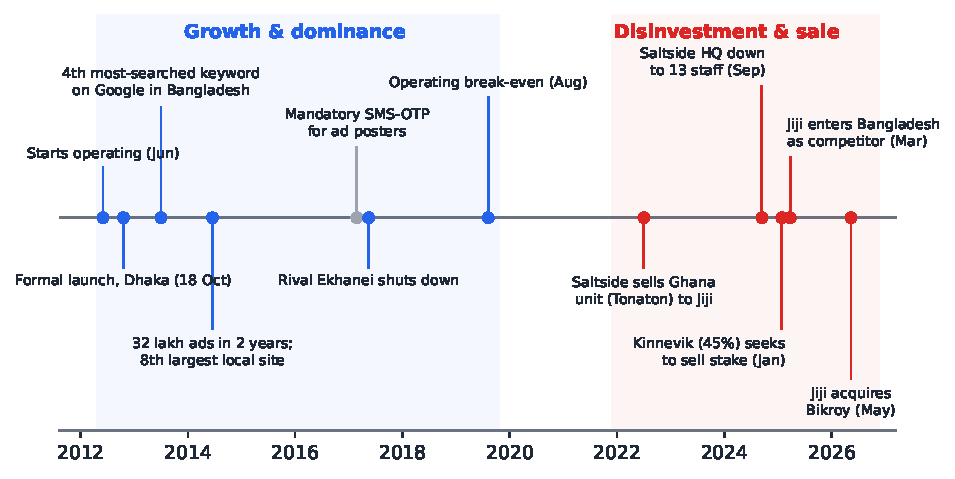
\includegraphics[width=\textwidth]{fig1_timeline.pdf}
  \caption{Timeline of Bikroy.com, 2012--2026. Blue: growth milestones; red: events in the
  decline of its parent company and its eventual sale; grey: anti-fraud measures.
  Sources: \cite{wiki_bikroy,bn24_2014,fs_fraud,fs_ekhanei,fs_jiji,intellinews,ds_jiji}.}
  \label{fig:timeline}
\end{figure}

\subsection{Launch and rapid growth (2012--2014)}

Bikroy began operating in June 2012 and was formally launched at a press conference in
Dhaka on 18~October~2012. The Daily Star described it at the time as the country's first
bilingual (Bangla and English) classified website~\cite{wiki_bikroy}. It was owned by
Saltside Technologies, a Swedish company that also ran classifieds sites in Ghana (Tonaton)
and Sri Lanka (ikman)~\cite{fs_jiji}.

Growth in the first two years was very fast (Figure~\ref{fig:growth}). Bikroy received
26{,}000 advertisements in its first three months (June--August 2012), and 8.27~lakh
(827{,}000) in March--May 2014 alone, an increase of roughly 32 times. By June 2014 it had
received more than 32~lakh ads in total and was handling over 9{,}000 new ads per day,
compared with about 3{,}000 a year earlier~\cite{bn24_2014}. In the same period it became,
by Alexa ranking, the 8th largest local website in Bangladesh~\cite{bn24_2014}, and in 2013
``Bikroy.com'' was the 4th most-searched keyword on Google in Bangladesh~\cite{wiki_bikroy}.
In September 2014 the company stated that it received more than 2~million unique visitors
per month~\cite{fe_2014}.

\begin{figure}[H]
  \centering
  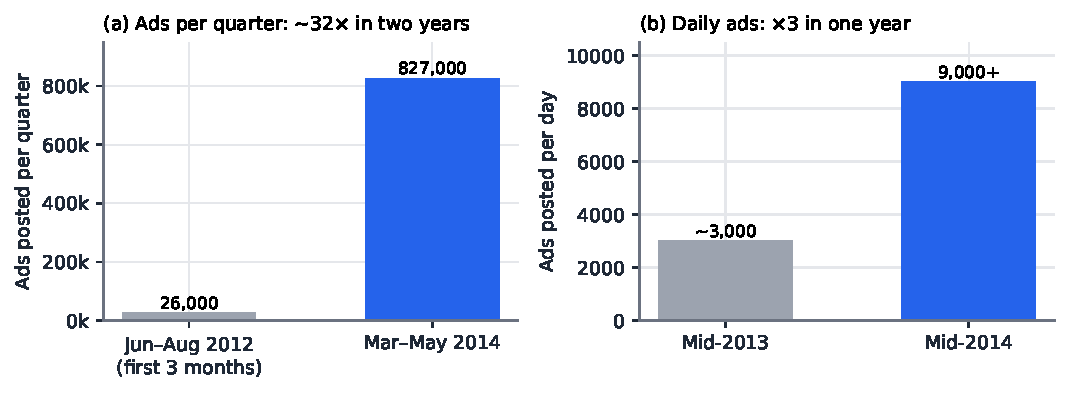
\includegraphics[width=\textwidth]{fig2_early_growth.pdf}
  \caption{Bikroy's early growth. (a) Ads posted per quarter in the first quarter of
  operation and in March--May 2014. (b) Ads posted per day, mid-2013 vs.\ mid-2014.
  Source: Banglanews24~\cite{bn24_2014}.}
  \label{fig:growth}
\end{figure}

\paragraph{Fraud was present from the start.} Rapid growth came with a trust problem that
Bikroy itself acknowledged. In September 2014, Bikroy's marketing manager told the Crime
Reporters Association of Bangladesh that in a random sample of 500 ads, only 330 (66\%)
were genuine; some advertisers did not respond when their listed numbers were called
(Figure~\ref{fig:genuine}). She added that fake sellers typically priced items below
market and, in many cases, lured buyers to remote locations and robbed them. Bikroy's
investigation team removed more than 750 fake ads in August 2014 alone~\cite{dt_2014}.

\begin{figure}[H]
  \centering
  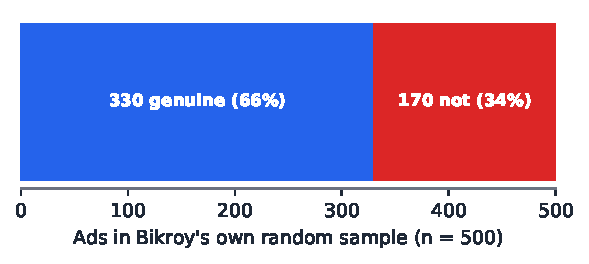
\includegraphics[width=0.68\textwidth]{fig3_genuine_ads.pdf}
  \caption{Result of Bikroy's own 2014 audit of 500 randomly sampled ads: one in three
  was not genuine. Source: Dhaka Tribune~\cite{dt_2014}.}
  \label{fig:genuine}
\end{figure}

Note that the audit measured \emph{ads}, not victims: the 170 non-genuine ads in the sample
tell us how much of the catalogue could not be trusted, but Bikroy did not publish how many
buyers had actually lost money to them.

\paragraph{What Bikroy did about it.} Bikroy did respond, but every measure it took was
aimed at cleaning up \emph{listings}, not at protecting or compensating the people who
\emph{transacted} through them (Table~\ref{tab:response}).

\begin{table}[H]
  \centering
  \small
  \caption{Bikroy's documented responses to fraud, 2014--2026, and whether each one
  protects money in a transaction or helps a victim recover a loss.}
  \label{tab:response}
  \begin{tabularx}{\textwidth}{@{}l Y c c@{}}
    \toprule
    \textbf{When} & \textbf{Measure} & \textbf{Protects payment?} & \textbf{Helps victims recover?} \\
    \midrule
    Aug 2014 & Internal investigation team; 750+ fake ads removed in one month;
      press awareness event with crime reporters~\cite{dt_2014} & No & No \\
    2016 & ``Buy Now'': Bikroy-coordinated delivery with cash on delivery after
      inspection, for selected listings~\cite{fs_fraud,ds_buynow} & Partly & No \\
    Feb 2017 & Mandatory SMS one-time-password for new ad posters; ban on replica and
      clone products~\cite{fs_fraud} & No & No \\
    Ongoing & Ads reviewed before publication~\cite{ds_jiji}; full records kept on
      paying members, cited by Bikroy during a police case~\cite{ds_muktagacha} & No & Indirectly \\
    2026 & Safety-tips page: check seller feedback, avoid prepayment, inspect before
      paying; no escrow, payment protection or refund process~\cite{bikroy_safety} & No & No \\
    \bottomrule
  \end{tabularx}
\end{table}

\paragraph{No compensation, by design.} We found no public record of Bikroy refunding or
compensating any fraud victim, at any point from 2012 to 2026. This is not an oversight
but the platform's stated policy. Bikroy's current Terms and Conditions (operated by Bikroy
Marketplace Ltd., last updated 17~April~2026) state that the platform is not a party to
transactions between users, accept no responsibility for loss or damage arising from user
interactions, place the duty of due diligence on the user, and cap Bikroy's total liability
at the lesser of the fees the user paid in the previous six months or BDT~6{,}700. Fees paid
for promotion are non-refundable~\cite{bikroy_terms}. A buyer who sends a 50{,}000-taka
advance to a fake seller therefore has no recourse against Bikroy; the only route is a
police case against the scammer, as in the Muktagacha case, where Bikroy's public role was limited
to pointing to the records it keeps on paying members and checking whether any of its own
staff or courier employees were involved~\cite{ds_muktagacha}.

\paragraph{The audit was never repeated publicly.} The 2014 figure of 66\% genuine ads is
the only fraud-rate measurement Bikroy appears to have ever published. We found no later
audit, no annual trust-and-safety report, and no statement of how the genuine-ad rate
changed after the 2017 measures. Bikroy's later public statements on fraud are general
assurances, such as that ads are reviewed before publication~\cite{ds_jiji}, rather than
measured results, while fraud on the platform continues to surface in police reporting of
individual scams (Section~\ref{sec:downfall}). Without a published follow-up, there is no evidence that the
problem identified in 2014 was ever measured as solved.

\subsection{Market dominance (2015--2019)}

Bikroy did not win its market by out-competing rivals on trust; it won by outlasting them.
Ekhanei (formerly CellBazaar, owned by Telenor, Schibsted and Naspers, and merged with OLX
Bangladesh in 2015) shut down on 17~May~2017, with its owners stating that they had been
unable to build a sustainable, profitable business~\cite{fs_ekhanei}. With its main rival
gone, Bikroy became the clear market leader.

During this period Bikroy added a membership programme for small businesses (2016), a
``Buy Now'' service with partner couriers and cash-on-delivery after inspection, and, in
February 2017, mandatory SMS one-time-password verification for new ad posters together
with a ban on replica products~\cite{wiki_bikroy,ds_buynow,fs_fraud}. Future Startup noted at the time
that there was ``a widespread allegation against Bikroy for allowing fake
products''~\cite{fs_fraud}. In August 2019 Bikroy reached operating break-even for the
first time~\cite{wiki_bikroy,fs_jiji}.

Saltside's last institutional funding round, a \$40 million Series~B from Kinnevik,
Hillhouse Capital and Brummer \& Partners, closed in January 2015~\cite{fs_jiji}. As
Figure~\ref{fig:saltside} shows, no new capital followed for more than a decade.

\subsection{Bikroy in 2026: still large, but losing position}
\label{sec:present}

Bikroy has not collapsed. At the time of its sale in May 2026 it reported over 10~million
app downloads, about 400{,}000 monthly buyers, more than 100{,}000 monthly sellers,
roughly 3~million unique monthly visitors, 420 employees, and more than \$3~billion in
annual gross merchandise value (GMV)~\cite{fs_jiji}. That GMV is concentrated in
high-value categories, mainly vehicles and real estate~\cite{fs_jiji}. Table~\ref{tab:then_now}
compares its position then and now.

\begin{table}[H]
  \centering
  \small
  \caption{Bikroy.com then and now. Third-party traffic figures are estimates and are not
  directly comparable with company-reported figures.}
  \label{tab:then_now}
  \begin{tabularx}{\textwidth}{@{}l Y Y@{}}
    \toprule
    \textbf{Indicator} & \textbf{2013--2014} & \textbf{2025--2026} \\
    \midrule
    Rank in Bangladesh & 8th largest local site (Alexa)~\cite{bn24_2014}
      & \#67 (Similarweb, Sep 2026)~\cite{similarweb_2026}; \#104 (Semrush, Aug 2026)~\cite{semrush_2026} \\
    Monthly audience & 2.0M+ unique visitors (company, 2014)~\cite{fe_2014}
      & $\sim$3M unique visitors (company, 2026)~\cite{fs_jiji}; 3.3M total visits in the last three months (Similarweb, Jul--Sep 2026)~\cite{similarweb_2026} \\
    Traffic trend & Ads $\times$32 in two years~\cite{bn24_2014}
      & $-18.93\%$ MoM (Dec 2025, Semrush)~\cite{semrush_2025}; $-12.78\%$ MoM (Sep 2026, Similarweb)~\cite{similarweb_2026} \\
    Owner & Saltside Technologies, actively funded (\$40M, Jan 2015)~\cite{fs_jiji}
      & Jiji (Nigeria), acquired May 2026~\cite{ds_jiji} \\
    User trust & Only 66\% of sampled ads genuine~\cite{dt_2014}
      & Trustpilot score 2.0/5 (13 reviews)~\cite{trustpilot} \\
    \bottomrule
  \end{tabularx}
\end{table}

\paragraph{Ranking.} Bikroy has fallen from a top-ten local website in 2014 to between
\#67 and \#104 among all websites visited in Bangladesh in 2026, depending on the analytics
provider (Figure~\ref{fig:rank}). The two measures are not identical (Alexa's 2014 figure
ranked \emph{local} sites, whereas today's figures rank all sites, including Google,
Facebook and YouTube), so the size of the fall should not be overstated, but the direction
is clear.

\begin{figure}[H]
  \centering
  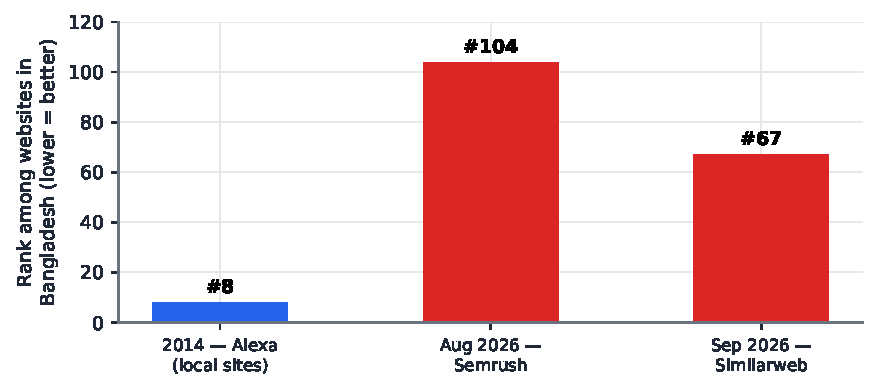
\includegraphics[width=0.78\textwidth]{fig4_bd_rank.pdf}
  \caption{Bikroy's website rank in Bangladesh, 2014 vs.\ 2026. The 2014 figure is
  Alexa's ranking among local websites; the 2026 figures rank all websites. Sources:
  \cite{bn24_2014,semrush_2026,similarweb_2026}.}
  \label{fig:rank}
\end{figure}

\paragraph{Recent traffic.} Both independent analytics providers we checked report
month-on-month declines: Semrush estimated 1.35~million visits in December 2025, down
18.93\% from November~\cite{semrush_2025}, and Similarweb reported a 12.78\% month-on-month
fall for September 2026, with Bikroy's global rank slipping from \#10{,}746 to \#12{,}370
over three months~\cite{similarweb_2026} (Figure~\ref{fig:traffic}). Single-month changes
can reflect seasonality, so these figures indicate softening rather than proof of a
long-term trend.

\begin{figure}[H]
  \centering
  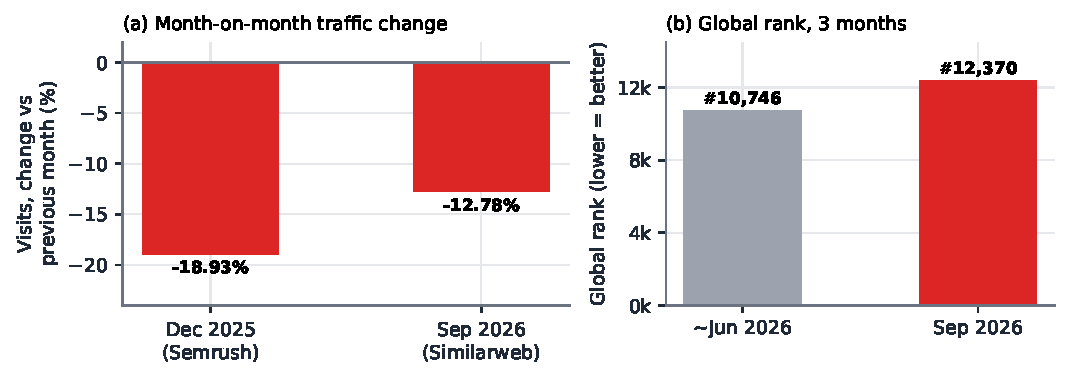
\includegraphics[width=\textwidth]{fig5_recent_traffic.pdf}
  \caption{Recent traffic signals. (a) Month-on-month change in visits reported by
  Semrush (December 2025) and Similarweb (September 2026). (b) Similarweb global rank
  at the start and end of the three months to September 2026. Sources:
  \cite{semrush_2025,similarweb_2026}.}
  \label{fig:traffic}
\end{figure}

\subsection{What Bikroy sells and how many people use it}
\label{sec:catalogue}

\paragraph{Most ads are everyday used goods.} A snapshot of Bikroy's category pages on
7~October~2026 counted 296{,}743 live ads on the site as a whole; the 17 top-level categories
sum to 300{,}635, a difference of about 1\% that reflects ads being added and removed while
the pages were read~\cite{bikroy_cats}. Figure~\ref{fig:cat_counts} shows the breakdown.
Phones and tablets (85{,}553 ads, 28.5\%) and electronics (57{,}170, 19.0\%) together make up
almost half of all listings, followed by home, furniture and appliances (32{,}892, 10.9\%).
Vehicles (29{,}987, 10.0\%) and property (14{,}242, 4.7\%) together account for only about
15\% of ads.

\begin{figure}[H]
  \centering
  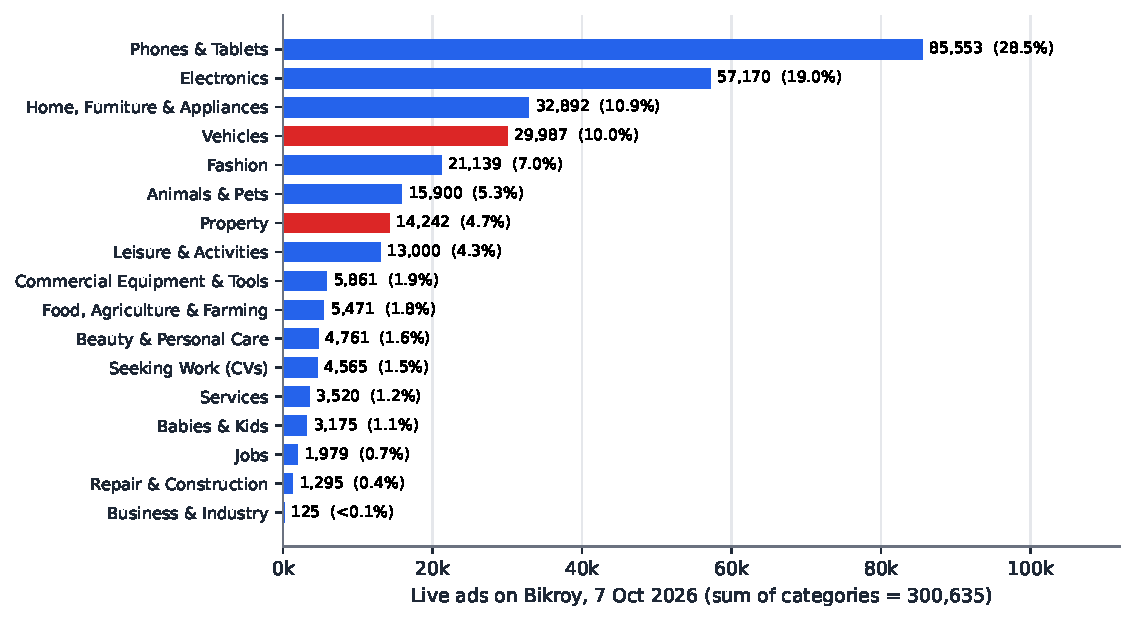
\includegraphics[width=\textwidth]{fig_cat_counts.pdf}
  \caption{Live ads on Bikroy by top-level category, 7~October~2026. Red: the two high-value
  categories (vehicles and property); blue: all others. Percentages are shares of the sum of
  categories. Source: Bikroy category pages~\cite{bikroy_cats}.}
  \label{fig:cat_counts}
\end{figure}

\paragraph{And they are mostly second-hand.} The condition filters show that Bikroy is still
overwhelmingly a market for used goods (Figure~\ref{fig:used_share}). Of 75{,}392 mobile-phone
ads, 68{,}360 (91\%) are for used phones, 1{,}528 (2\%) refurbished and 5{,}303 (7\%) new. Of
20{,}717 laptop and computer ads, 18{,}308 (88\%) are used, 257 (1\%) refurbished and 2{,}130
(10\%) new~\cite{bikroy_cats}. In 2017 Bikroy's marketing director said that about a quarter
of goods traded on the site were new items sold by small retailers~\cite{fs_b2b}; that figure
measured trades rather than listings, so it is not directly comparable, but both point the
same way: most of what changes hands on Bikroy is second-hand.

\begin{figure}[H]
  \centering
  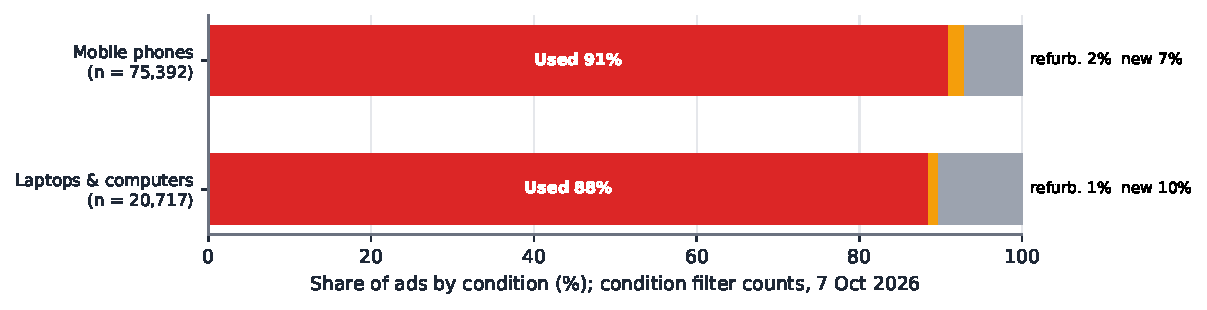
\includegraphics[width=0.92\textwidth]{fig_used_share.pdf}
  \caption{Share of ads by condition in Bikroy's two largest everyday-goods subcategories,
  7~October~2026. Source: Bikroy condition filters~\cite{bikroy_cats}.}
  \label{fig:used_share}
\end{figure}

\paragraph{Listings versus value.} These counts do not contradict the report at the time of the
sale that Bikroy's \$3~billion annual GMV is concentrated in vehicles and real
estate~\cite{fs_jiji}. A single flat or car is worth as much as hundreds of used phones, so the
two high-value categories can dominate the money while everyday goods dominate the ads. Bikroy
therefore still sells old goods in large numbers: by number of listings it is mainly a
second-hand phone, electronics and household-goods market, while by value it is mainly a car
and property market. The person-to-person resale of used goods, where the scams documented in
Section~\ref{sec:users} occur, is the largest part of its catalogue.

\paragraph{Digital goods.} Bikroy's video-games subcategory held 288 ads in the same snapshot,
including game-account sales such as Free Fire and eFootball IDs priced at BDT~7{,}000 to
32{,}500~\cite{bikroy_cats}. This trade is discussed in Section~\ref{sec:facebook}.

\paragraph{How many people use Bikroy.} Bikroy does not publish a yearly traffic series, so
visitor numbers over time have to be pieced together from occasional company statements and
third-party estimates. The company figures use the same measure, monthly unique visitors or
users, and are shown in Figure~\ref{fig:audience}: more than 2~million in September
2014~\cite{fe_2014}, around 2~million in March 2017~\cite{fs_b2b}, and about 3~million at the
time of the sale in May 2026~\cite{fs_jiji}. Taken at face value, the audience grew by roughly
half over twelve years, and was essentially flat between 2014 and 2017.

\begin{figure}[H]
  \centering
  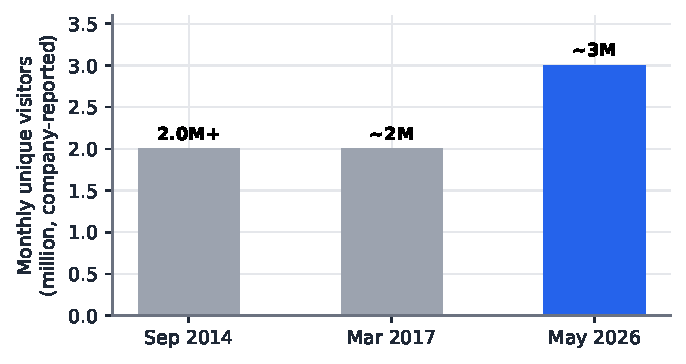
\includegraphics[width=0.62\textwidth]{fig_audience_years.pdf}
  \caption{Bikroy's monthly audience as reported by the company at three points in time.
  Sources: \cite{fe_2014,fs_b2b,fs_jiji}.}
  \label{fig:audience}
\end{figure}

Third-party estimates measure total visits rather than unique visitors, and they disagree
sharply with each other (Table~\ref{tab:traffic_est}). Semrush's two estimates eight months
apart differ by a factor of about nine, which reflects changes in estimation rather than a
real ninefold jump. These figures are therefore used in this report only for direction of
change over short periods (Figure~\ref{fig:traffic}), not for the size of Bikroy's audience.

\begin{table}[H]
  \centering
  \small
  \caption{Third-party traffic estimates for bikroy.com. Estimates from different providers, or
  from the same provider at different times, are not directly comparable.}
  \label{tab:traffic_est}
  \begin{tabularx}{\textwidth}{@{}l l Y@{}}
    \toprule
    \textbf{Provider} & \textbf{Period} & \textbf{Estimate} \\
    \midrule
    Semrush & Dec 2025 & 1.35~million visits, down 18.93\% on the previous month~\cite{semrush_2025} \\
    Semrush & Aug 2026 & 12.4~million visits~\cite{semrush_2026} \\
    Similarweb & Jul--Sep 2026 & 3.3~million visits over three months (about 1.1~million a month);
      down 12.78\% in September~\cite{similarweb_2026} \\
    \bottomrule
  \end{tabularx}
\end{table}

\subsection{Owner retreat and sale (2022--2026)}
\label{sec:sale}

The clearest sign of decline is not in Bikroy's own numbers but in its owner's behaviour
(Figure~\ref{fig:saltside}). Saltside sold its Ghanaian platform, Tonaton, to Jiji in 2022.
By September 2024, Saltside's group-level headcount had fallen to 13 people. In January
2025, Kinnevik, Saltside's largest shareholder with a 45\% stake, publicly announced it
wanted to sell that stake~\cite{fs_jiji}. Two months later, in March 2025, the Nigerian
classifieds company Jiji entered Bangladesh through \texttt{jiji-bd.com} as a direct
competitor to Bikroy, Daraz and Ajkerdeal~\cite{intellinews}. Thirteen months after that,
in May 2026, Jiji acquired Bikroy~\cite{ds_jiji,intellinews}.

\begin{figure}[H]
  \centering
  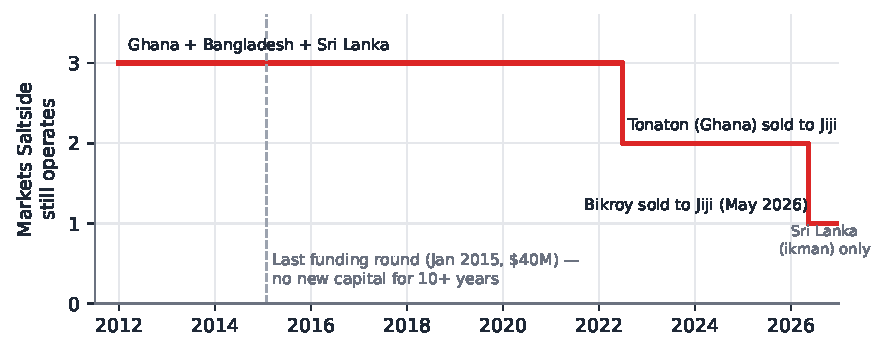
\includegraphics[width=0.85\textwidth]{fig6_saltside.pdf}
  \caption{Number of markets in which Saltside Technologies still operates a classifieds
  platform. After its last funding round in January 2015, it sold Ghana (2022) and
  Bangladesh (2026), both to Jiji. Source: Future Startup~\cite{fs_jiji}.}
  \label{fig:saltside}
\end{figure}

Under Jiji, the Bikroy brand will survive, but the platform is being moved onto Jiji's
technology and its monetisation is changing from Bikroy's flat-fee model to a
pay-per-click bidding system in which sellers bid for placement~\cite{fs_jiji}. Future
Startup observes that this changes the economics for small sellers significantly,
because it favours sellers with larger budgets and the skill to optimise bids~\cite{fs_jiji}.
After the acquisition, Jiji's main competition in Bangladesh is Facebook Marketplace and
social-media sellers~\cite{fs_jiji}.

\subsection{Causes of decline}
\label{sec:downfall}

Bikroy is still a large, functioning business, so ``downfall'' here means a loss of
momentum, market position and independence rather than a collapse. The evidence above
points to six connected causes.

\begin{enumerate}[label=\textbf{\arabic*.}]
  \item \textbf{The trust problem was managed, never solved.} Bikroy's own 2014 audit found
  that one ad in three was not genuine~\cite{dt_2014}. Its main response, SMS-OTP
  verification in 2017~\cite{fs_fraud}, only proves control of a phone number, and police
  later broke up a gang that bought registered SIM cards for 350--500 taka each to post
  fake electronics ads on Bikroy~\cite{ds_muktagacha}. In 2026, Bikroy's listing pages
  still tell users to avoid advance payment, meet in a public place and pay only after
  inspection~\cite{bikroy_listing}; the responsibility for safety remains with the user.

  \item \textbf{It never controlled the transaction.} Bikroy connects buyers and sellers
  but, outside its ``Buy Now'' cash-on-delivery service, payment and handover happen
  off-platform. A platform that does not hold the money cannot protect either party, and
  cash meetings expose both sides to fraud, as in the 2023 case where a gang paid an
  iPhone seller who had advertised on Bikroy with a bundle of mostly 20-taka notes
  disguised as 1{,}000-taka notes~\cite{pa_2023}.

  \item \textbf{It won by default, not by innovation.} Bikroy's dominance came after
  well-funded rivals exited~\cite{fs_ekhanei}, and Future Startup notes it ``didn't face
  much sustained competition''~\cite{fs_jiji}. Without competitive pressure, the core
  model (a listing board) stayed essentially the same for over a decade.

  \item \textbf{Its owner stopped investing.} Saltside raised no new capital after January
  2015, shrank its headquarters to 13 people, sold Ghana, and saw its largest shareholder
  seek an exit~\cite{fs_jiji}. A platform whose owner is looking for the door does not make
  bold new bets on trust infrastructure.

  \item \textbf{Its audience is being absorbed by social media.} In an interview with Future Startup, Bikroy's
  marketing director called Facebook the biggest challenge for every online site in
  Bangladesh~\cite{fs_misha}. Today Jiji itself names Facebook Marketplace and
  social-media sellers as Bikroy's main competition~\cite{fs_jiji}, and third-party
  traffic estimates show Bikroy losing rank (Figures~\ref{fig:rank} and~\ref{fig:traffic}).

  \item \textbf{Small individual sellers are being priced toward the margins.} The switch
  to pay-per-click bidding favours businesses with marketing budgets~\cite{fs_jiji}, and
  sellers already complain that paid promotion produces fake inquiries rather than
  buyers~\cite{trustpilot}. Most of Bikroy's transaction value is in cars and
  property~\cite{fs_jiji}, yet most of its ads are everyday used goods posted by individuals
  (Section~\ref{sec:catalogue}). The pricing change falls hardest on exactly the sellers who
  make up the bulk of its catalogue.
\end{enumerate}

\paragraph{Implication for TrustBazaar.} Bikroy has not been ``replaced'' because every
challenger (OLX, Ekhanei and Jiji) competed with the same model: a listing board where
payment and delivery happen elsewhere. None competed on the transaction itself. The gap
that remains, verified identity, money held until delivery, fair price discovery and
coordinated delivery for individual-to-individual resale, is exactly the space TrustBazaar
targets. TrustBazaar does not need to out-list Bikroy; it needs to make the transactions
that Bikroy leaves to chance safe.

\section{Users' Experience and Fraud on Bikroy.com}
\label{sec:users}

Section~\ref{sec:history} showed that Bikroy remains large but has never solved its trust
problem. This section examines what buyers and sellers actually experience on Bikroy,
whether people are still being scammed, and where exactly in a transaction the platform
leaves them exposed. We separate two things that are often
confused: how users rate the \emph{app} as a tool, and how safe a \emph{transaction} made
through it is.

\subsection{What users say}

\paragraph{The app itself is well liked.} It would be misleading to claim users hate Bikroy.
On Google Play, the Bikroy app has a 4.3-star average from about 210{,}000 reviews and more
than 10~million downloads (Figure~\ref{fig:ratings})~\cite{play_store}. People value it as a
fast way to post an ad and reach buyers. The most visible recent reviews (May--September
2026) complain mainly about usability after the switch to Jiji's platform: users report that
the redesigned interface is harder to navigate and that the filter separating member
(business) ads from individual sellers was removed, making person-to-person deals and price
comparison harder~\cite{play_store}.

\paragraph{Sellers who pay are less satisfied.} On Trustpilot, Bikroy scores 2.0 out of 5
from 13 reviews~\cite{trustpilot}. One seller advised others never to pay for ads, suspecting
that paid promotions trigger automated messages that only look like buyer interest; the same
reviewer objected to manual review and requests for private information on a flat-rental
ad~\cite{trustpilot}. Thirteen reviews is far too few to represent all users, so we treat
these as illustrative complaints rather than a measurement.

\begin{figure}[H]
  \centering
  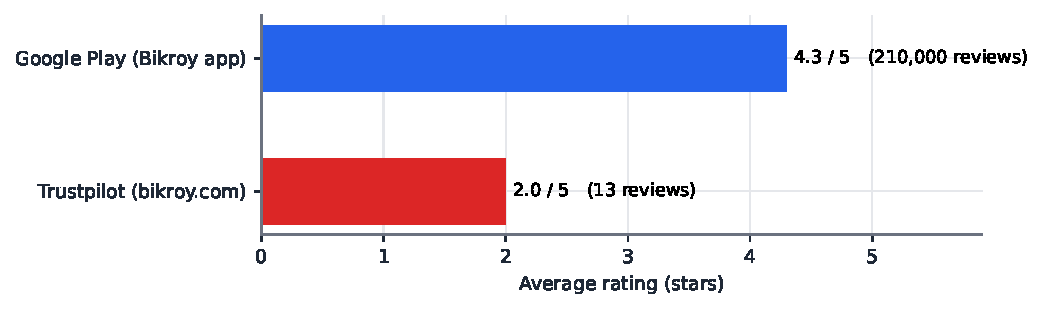
\includegraphics[width=0.85\textwidth]{fig7_ratings.pdf}
  \caption{Bikroy's ratings on two review platforms, as of October 2026. The very different
  sample sizes mean the two numbers measure different things: app usability for a large
  general audience versus experiences of a small, self-selected group.
  Sources: \cite{play_store,trustpilot}.}
  \label{fig:ratings}
\end{figure}

\paragraph{Why ratings do not measure safety.} A high app rating and a high scam risk can
coexist. App-store reviews are written mostly by people for whom the app worked; a buyer who
loses money to a fake seller blames the seller or the police process, not the app's
interface. National data show how rarely fraud victims take formal action at all: in a
2023--24 survey of 132 cybercrime victims by the Cyber Crime Awareness Foundation (CCAF),
40.15\% had suffered financial loss, but only 12\% pursued legal action
(Figure~\ref{fig:ccaf})~\cite{ccaf_2024}. Most fraud, in other words, is never recorded
anywhere a researcher can find it.

\begin{figure}[H]
  \centering
  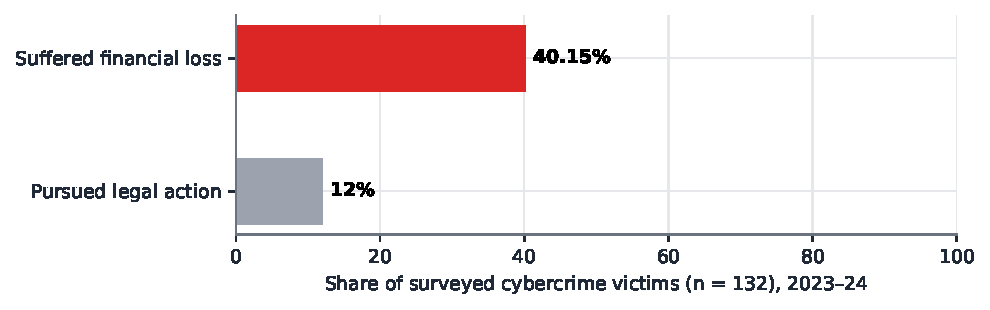
\includegraphics[width=0.85\textwidth]{fig8_ccaf.pdf}
  \caption{Financial loss versus legal action among 132 surveyed cybercrime victims in
  Bangladesh (survey period April 2023 -- April 2024). Source: CCAF~\cite{ccaf_2024}.}
  \label{fig:ccaf}
\end{figure}

\subsection{Documented scams and how they work}

Police and newspaper reports describe a small number of recurring scam patterns on Bikroy.
Table~\ref{tab:scams} classifies them by who is harmed and at which stage of the
transaction.

\begin{table}[H]
  \centering
  \small
  \caption{Scam patterns documented on Bikroy.com.}
  \label{tab:scams}
  \begin{tabularx}{\textwidth}{@{}>{\raggedright\arraybackslash}p{2.7cm} >{\raggedright\arraybackslash}p{1.3cm} >{\raggedright\arraybackslash}p{1.9cm} Y@{}}
    \toprule
    \textbf{Pattern} & \textbf{Victim} & \textbf{Stage} & \textbf{Evidence} \\
    \midrule
    Fake seller, advance payment & Buyer & Payment
      & Muktagacha gang posted cheap phone and electronics ads from accounts opened with
        SIM cards bought for Tk~350--500; took lakhs of taka~\cite{ds_muktagacha}.
        Fake sellers typically underprice items~\cite{dt_2014}. \\
    Lure and robbery & Buyer & Handover
      & In 2014 Bikroy itself reported fake sellers luring buyers to remote places and
        robbing them~\cite{dt_2014}. \\
    Fake buyer, counterfeit or swapped cash & Seller & Payment and handover
      & 2023: gang paid an iPhone seller with a bundle of mostly Tk~20 notes; active for
        more than three years; three arrested~\cite{pa_2023}. \\
    Fake or replica goods & Buyer & Listing
      & Widespread allegations by 2017 led Bikroy to ban replica and clone
        items~\cite{fs_fraud}. \\
    Fake inquiries after paid promotion & Seller & Listing
      & Seller complaint that paid ads attract automated, non-genuine
        messages~\cite{trustpilot} (unverified, single review). \\
    \bottomrule
  \end{tabularx}
\end{table}

Two of these patterns are traced step by step below. Figure~\ref{fig:advance} shows the
fake-seller scam as reconstructed from the Muktagacha case and Bikroy's own 2014 account.
Each check Bikroy runs (phone verification and ad review) happens \emph{before} the scam
starts; once buyer and seller are talking directly, the money moves entirely outside the
platform, and afterwards Bikroy's terms state that it is not a party to the
transaction~\cite{bikroy_terms}.

\begin{figure}[H]
  \centering
  \resizebox{0.97\textwidth}{!}{% Fake-seller / advance-payment scam, compiled from documented cases
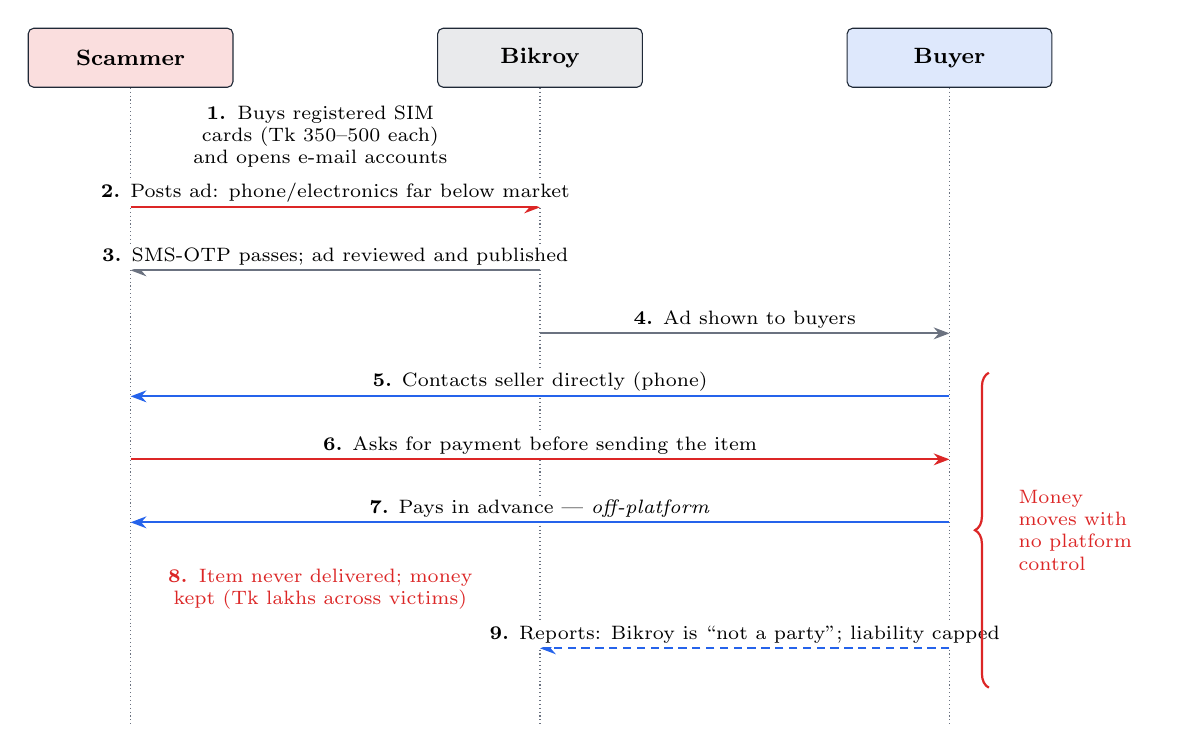
\begin{tikzpicture}[
  font=\footnotesize,
  actor/.style={draw=ink, fill=#1!15, rounded corners=2pt, minimum width=2.6cm,
                minimum height=0.75cm, font=\footnotesize\bfseries},
  life/.style={draw=muted, densely dotted},
  msg/.style={-{Stealth[length=2mm]}, thick, draw=#1},
  lab/.style={font=\scriptsize, fill=white, inner sep=1.5pt, align=center}]

  \node[actor=bad]   (S) at (0,0)   {Scammer};
  \node[actor=muted] (B) at (5.2,0) {Bikroy};
  \node[actor=good]  (V) at (10.4,0){Buyer};
  \foreach \n in {S,B,V}{ \draw[life] (\n.south) -- ++(0,-8.1); }

  % 1
  \node[lab, anchor=west, text width=4.4cm] at (0.15,-1.0)
    {\textbf{1.} Buys registered SIM cards (Tk 350--500 each) and opens e-mail accounts};
  % 2
  \draw[msg=bad] (0,-1.9) -- node[lab, above]{\textbf{2.} Posts ad: phone/electronics far below market} (5.2,-1.9);
  % 3
  \draw[msg=muted] (5.2,-2.7) -- node[lab, above]{\textbf{3.} SMS-OTP passes; ad reviewed and published} (0,-2.7);
  % 4
  \draw[msg=muted] (5.2,-3.5) -- node[lab, above]{\textbf{4.} Ad shown to buyers} (10.4,-3.5);
  % 5
  \draw[msg=good] (10.4,-4.3) -- node[lab, above]{\textbf{5.} Contacts seller directly (phone)} (0,-4.3);
  % 6
  \draw[msg=bad] (0,-5.1) -- node[lab, above]{\textbf{6.} Asks for payment before sending the item} (10.4,-5.1);
  % 7
  \draw[msg=good] (10.4,-5.9) -- node[lab, above]{\textbf{7.} Pays in advance --- \emph{off-platform}} (0,-5.9);
  % 8
  \node[lab, anchor=west, text width=4.4cm, text=bad] at (0.15,-6.75)
    {\textbf{8.} Item never delivered; money kept (Tk lakhs across victims)};
  % 9
  \draw[msg=good, densely dashed] (10.4,-7.5) -- node[lab, above]{\textbf{9.} Reports: Bikroy is ``not a party''; liability capped} (5.2,-7.5);

  % bracket: Bikroy never touches the money
  \draw[decorate, decoration={brace, amplitude=5pt, mirror}, thick, bad]
    (10.9,-4.0) -- (10.9,-8.0)
    node[midway, right=7pt, font=\scriptsize, text=bad, align=left, text width=1.6cm]
    {Money moves with no platform control};
\end{tikzpicture}
}
  \caption{Typical fake-seller (advance-payment) scam on a classifieds platform, compiled
  from the Muktagacha case~\cite{ds_muktagacha}, Bikroy's 2014 statement~\cite{dt_2014} and
  Bikroy's current terms~\cite{bikroy_terms}. Steps 3--4 are the only points at which the
  platform is involved.}
  \label{fig:advance}
\end{figure}

Figure~\ref{fig:noteswap} shows the reverse case, where the \emph{seller} is the victim.
This scam does not need a fake listing at all: it exploits the cash meeting that Bikroy's
own safety advice recommends (meet in person, inspect, then pay)~\cite{bikroy_safety}.

\begin{figure}[H]
  \centering
  \resizebox{0.97\textwidth}{!}{% Fake-buyer counterfeit/note-swap scam (Prothom Alo, 2023)
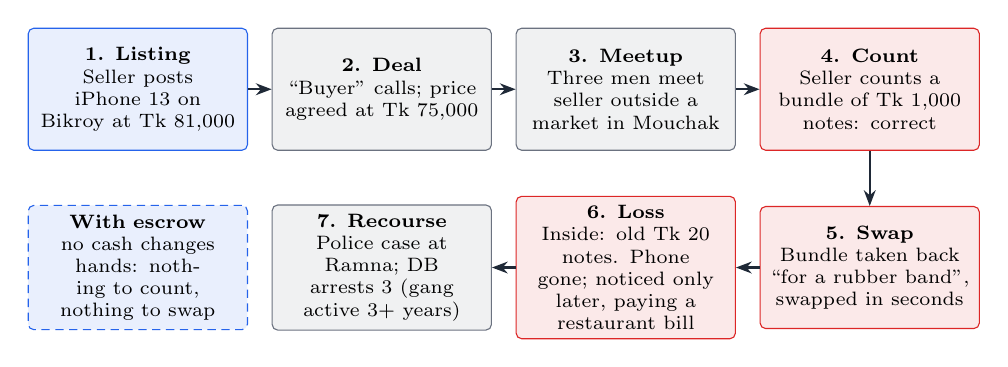
\begin{tikzpicture}[
  font=\footnotesize, node distance=3mm,
  step/.style={draw=#1, fill=#1!10, rounded corners=2pt, text width=2.55cm,
               minimum height=1.55cm, align=center, font=\scriptsize},
  flow/.style={-{Stealth[length=2mm]}, thick, draw=ink}]

  \node[step=good]                 (a) {\textbf{1. Listing}\\Seller posts iPhone~13 on Bikroy at Tk~81,000};
  \node[step=muted, right=of a]    (b) {\textbf{2. Deal}\\``Buyer'' calls; price agreed at Tk~75,000};
  \node[step=muted, right=of b]    (c) {\textbf{3. Meetup}\\Three men meet seller outside a market in Mouchak};
  \node[step=bad, right=of c]      (d) {\textbf{4. Count}\\Seller counts a bundle of Tk~1,000 notes: correct};
  \node[step=bad, below=7mm of d]  (e) {\textbf{5. Swap}\\Bundle taken back ``for a rubber band'', swapped in seconds};
  \node[step=bad, left=of e]       (f) {\textbf{6. Loss}\\Inside: old Tk~20 notes. Phone gone; noticed only later, paying a restaurant bill};
  \node[step=muted, left=of f]     (g) {\textbf{7. Recourse}\\Police case at Ramna; DB arrests 3 (gang active 3+ years)};
  \node[step=good, left=of g, draw=good, fill=good!10, densely dashed]
                                   (h) {\textbf{With escrow}\\no cash changes hands: nothing to count, nothing to swap};

  \draw[flow] (a) -- (b); \draw[flow] (b) -- (c); \draw[flow] (c) -- (d);
  \draw[flow] (d) -- (e); \draw[flow] (e) -- (f); \draw[flow] (f) -- (g);
\end{tikzpicture}
}
  \caption{The 2023 note-swap scam against a seller who listed an iPhone~13 on Bikroy,
  reconstructed from Prothom Alo's report of the Detective Branch case~\cite{pa_2023}. The
  dashed box shows what an escrow payment would remove.}
  \label{fig:noteswap}
\end{figure}

\subsection{Where Bikroy's protection stops}

Putting the cases together gives a clear picture (Figure~\ref{fig:lifecycle}). A used-goods
deal passes through six stages. Bikroy has weak control over the first three (identity,
listing, contact) and none over the last three (payment, handover, dispute). The most
damaging documented scams (fake sellers, robbery and counterfeit cash) strike in the three
stages Bikroy does not control, while fake identities and replica goods pass through the weak
checks at the start.

\begin{figure}[H]
  \centering
  \resizebox{\textwidth}{!}{% Where Bikroy's protection stops along a used-goods transaction
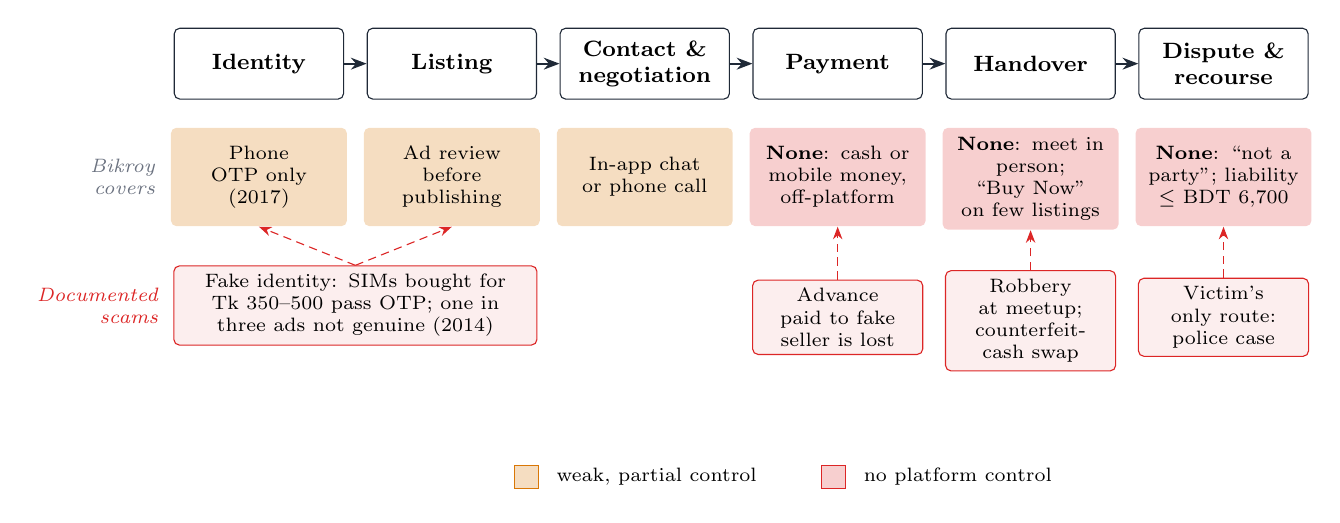
\begin{tikzpicture}[
  font=\footnotesize,
  stage/.style={draw=ink, fill=white, rounded corners=2pt, minimum width=2.15cm,
                minimum height=0.9cm, align=center, font=\footnotesize\bfseries},
  cover/.style={rounded corners=2pt, minimum width=2.15cm, minimum height=1.25cm,
                align=center, text width=2.0cm, font=\scriptsize},
  hit/.style={draw=bad, fill=bad!8, rounded corners=2pt, align=center,
              font=\scriptsize, inner sep=3pt},
  flow/.style={-{Stealth[length=2mm]}, draw=ink, thick}]

  % stages
  \foreach \i/\name in {1/Identity, 2/Listing, 3/Contact \&\\negotiation,
                        4/Payment, 5/Handover, 6/Dispute \&\\recourse}{
    \node[stage] (s\i) at ({(\i-1)*2.45},0) {\name};
  }
  \foreach \a/\b in {1/2,2/3,3/4,4/5,5/6}{ \draw[flow] (s\a) -- (s\b); }

  % Bikroy's coverage at each stage
  \node[cover, fill=partial!25] (c1) [below=0.35cm of s1] {Phone OTP only\\(2017)};
  \node[cover, fill=partial!25] (c2) [below=0.35cm of s2] {Ad review before\\publishing};
  \node[cover, fill=partial!25] (c3) [below=0.35cm of s3] {In-app chat\\or phone call};
  \node[cover, fill=bad!22]     (c4) [below=0.35cm of s4] {\textbf{None}: cash or\\mobile money,\\off-platform};
  \node[cover, fill=bad!22]     (c5) [below=0.35cm of s5] {\textbf{None}: meet in\\person; ``Buy Now''\\on few listings};
  \node[cover, fill=bad!22]     (c6) [below=0.35cm of s6] {\textbf{None}: ``not a\\party''; liability\\$\le$ BDT 6,700};

  \node[anchor=east, font=\scriptsize\itshape, text=muted, align=right]
    at ([xshift=-2pt]c1.west) {Bikroy\\covers};

  % where documented scams strike
  \node[hit, text width=4.4cm] (h1) at ($(c1.south)!0.5!(c2.south)+(0,-1.0)$)
    {Fake identity: SIMs bought for Tk 350--500 pass OTP; one in three ads not genuine (2014)};
  \node[hit, text width=1.95cm] (h2) at ($(c4.south)+(0,-1.15)$)
    {Advance paid to fake seller is lost};
  \node[hit, text width=1.95cm] (h3) at ($(c5.south)+(0,-1.15)$)
    {Robbery at meetup; counterfeit-cash swap};
  \node[hit, text width=1.95cm] (h4) at ($(c6.south)+(0,-1.15)$)
    {Victim's only route: police case};
  \foreach \h/\c in {h1/c1,h1/c2,h2/c4,h3/c5,h4/c6}{
    \draw[-{Stealth[length=1.6mm]}, bad, densely dashed] (\h.north) -- (\c.south);
  }
  \node[anchor=east, font=\scriptsize\itshape, text=bad, align=right]
    at ([xshift=-2pt]h1.west) {Documented\\scams};

  % legend
  \node[draw=partial, fill=partial!25, minimum width=3mm, minimum height=3mm] (l1) at (3.4,-5.25) {};
  \node[right=1mm of l1, font=\scriptsize] {weak, partial control};
  \node[draw=bad, fill=bad!22, minimum width=3mm, minimum height=3mm] (l2) at (7.3,-5.25) {};
  \node[right=1mm of l2, font=\scriptsize] {no platform control};
\end{tikzpicture}
}
  \caption{Bikroy's control over each stage of a used-goods transaction (orange: weak or
  partial; red: none), and where the documented scams in Table~\ref{tab:scams} strike.
  Sources: \cite{fs_fraud,ds_jiji,bikroy_terms,bikroy_safety,ds_muktagacha,dt_2014,pa_2023}.}
  \label{fig:lifecycle}
\end{figure}

\subsection{Are people still being scammed in 2026?}
\label{sec:still}

We should be precise about what the evidence shows.

\begin{itemize}
  \item \textbf{Bikroy-named cases.} The police cases we found that explicitly name Bikroy
  run up to 2023~\cite{pa_2023,ds_muktagacha}. We did not find a 2025--26 news report that
  names Bikroy, but newspapers often describe the platform only as ``online'', so this is
  absence of reporting, not evidence that the scams stopped.
  \item \textbf{The platform's own position.} In 2026 every Bikroy listing still carries
  warnings to avoid advance payment and to meet in a public place~\cite{bikroy_listing}, and
  its terms still disclaim responsibility for losses between users~\cite{bikroy_terms}. The
  conditions that made these scams possible are unchanged.
  \item \textbf{The same pattern elsewhere.} Advance-payment fraud through online ads is
  still being prosecuted in 2026: in August 2026, police in Narail arrested members of a
  gang that took money through online ads for hilsa fish and recovered phones, SIM cards and
  Tk~60{,}000~\cite{itv_hilsa}.
\end{itemize}

\subsection{The national lesson: escrow already works}
\label{sec:escrowlesson}

Advance-payment fraud is not unique to Bikroy; it is one of the defining failures of
Bangladeshi online commerce. Evaly, which sold goods at half price against advance payment and then
failed to deliver, owed about Tk~543 crore to customers and suppliers; its founders were
sentenced in January 2025~\cite{bdnews_evaly}. A similar case against e-Orange was still
in court in February 2026~\cite{bdnews_eorange}.

The government's response was escrow. On 30~June~2021 Bangladesh Bank issued a circular
requiring payment gateways to hold customers' advance payments and release them to the
merchant only after the product is delivered and the delivery documents are
verified~\cite{tbs_escrow}. The effect was measurable (Figure~\ref{fig:escrow}): of
Tk~5.05~billion that customers paid through gateways from 14~October~2021, Tk~2.14~billion
was still being held when the failed platforms collapsed, and in October 2021 the government
decided to return it to customers who had not received their goods~\cite{fe_refund}.

\begin{figure}[H]
  \centering
  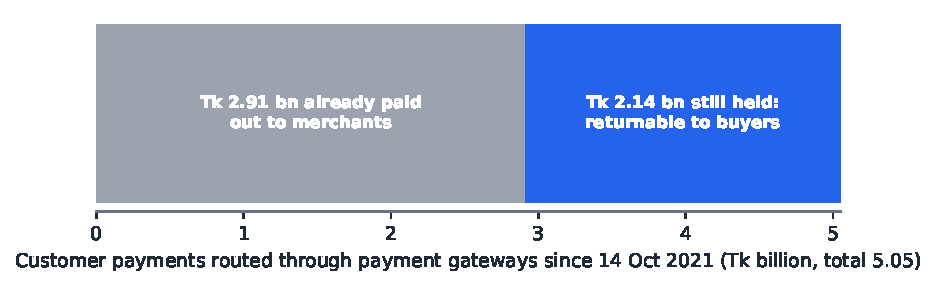
\includegraphics[width=0.9\textwidth]{fig9_escrow_funds.pdf}
  \caption{Customer payments routed through payment gateways under the 2021 escrow system,
  split into money already released to merchants and money still held, which could be
  returned to buyers. Source: The Financial Express~\cite{fe_refund}.}
  \label{fig:escrow}
\end{figure}

This regime protects buyers of \emph{business} e-commerce sites. It does not reach
person-to-person deals arranged through classifieds, because on Bikroy the payment never
passes through the platform or a gateway at all: buyer and seller settle in cash or by
direct transfer~\cite{bikroy_terms}. The protection Bangladesh already decided online buyers
need therefore stops exactly where individual resale begins.

\subsection{Summary: the loopholes}
\label{sec:loopholes}

The evidence in Sections~\ref{sec:history} and~\ref{sec:users} identifies six loopholes,
which Section~\ref{sec:solution} maps to TrustBazaar's features.

\begin{enumerate}[label=\textbf{L\arabic*.}]
  \item \textbf{Weak identity.} A phone number is the only identity check, and registered SIM
  cards can be bought for Tk~350--500~\cite{fs_fraud,ds_muktagacha}.
  \item \textbf{No payment protection.} Money moves off-platform with no holding
  point~\cite{bikroy_terms,bikroy_safety}.
  \item \textbf{Unsafe handover.} Buyers and sellers must meet with cash, which enables
  robbery and counterfeit-cash swaps~\cite{dt_2014,pa_2023}.
  \item \textbf{No recourse.} Bikroy is not a party to the deal, caps its liability at
  BDT~6{,}700 and offers no dispute process~\cite{bikroy_terms}.
  \item \textbf{No accountability record.} There is no verified transaction history, so a
  scammer can return under a new number, and Bikroy has published no fraud measurement since
  2014~\cite{dt_2014}.
  \item \textbf{No fair price discovery.} Bikroy offers fixed prices and informal
  negotiation only; there is no auction format with enforced rules.
\end{enumerate}

\section{How TrustBazaar Closes Bikroy's Loopholes}
\label{sec:solution}

Sections~\ref{sec:history} and~\ref{sec:users} showed that Bikroy's weakness is not its app,
which users rate 4.3 out of 5~\cite{play_store}, but the \emph{transaction}: Bikroy controls who
may post an ad, but not the money, the handover or the dispute, and its terms say
so~\cite{bikroy_terms}. This section takes the six loopholes identified in
Section~\ref{sec:loopholes} and shows, one by one, which TrustBazaar feature closes each and
how. It then replays the documented scams against TrustBazaar's design, and ends with a direct
answer to the question of why anyone would use it. All TrustBazaar features cited here are
specified in our project proposal~\cite{proposal}.

\subsection{Loophole-to-feature mapping}

Table~\ref{tab:mapping} pairs each loophole with the feature that closes it, and
Figure~\ref{fig:mapping} shows the full picture: which features act as the primary fix for each
loophole and which support it. Escrow settlement alone is the primary fix for three of the six
loopholes (L2, L3 and L4), which is why the proposal treats it as part of the critical
path~\cite{proposal}.

\begin{table}[!tbp]
  \centering
  \small
  \caption{Each Bikroy loophole (Section~\ref{sec:loopholes}) and the TrustBazaar feature that
  closes it. Objective (Obj.) and acceptance-criterion numbers refer to the project
  proposal~\cite{proposal}; requirement identifiers (FR-KYC, FR-AUC) refer to version~2.0 of the
  project's SRS.}
  \label{tab:mapping}
  \begin{tabularx}{\textwidth}{@{}>{\raggedright\arraybackslash}p{2.9cm}
                                  >{\raggedright\arraybackslash}p{3.3cm} Y@{}}
    \toprule
    \textbf{Loophole on Bikroy} & \textbf{TrustBazaar feature} & \textbf{How it closes the gap} \\
    \midrule
    \textbf{L1 Weak identity}: phone OTP only; SIM cards cost Tk~350--500~\cite{fs_fraud,ds_muktagacha}
      & NID + selfie KYC before listing or buying (Obj.~1; FR-KYC-01--FR-KYC-11), with an AI pre-check of
        document quality and selfie match
      & The account is tied to a verified national identity, not a SIM card. A banned person
        cannot return by buying a new number. \\
    \addlinespace
    \textbf{L2 No payment protection}: money moves off-platform~\cite{bikroy_terms,bikroy_safety}
      & Escrow settlement through bKash, Nagad or card (Obj.~3)
      & The buyer pays into escrow; the seller is paid only after the buyer confirms receipt, or
        automatically after a fixed timeout. This is the principle Bangladesh Bank mandated for
        e-commerce in 2021~\cite{tbs_escrow}. \\
    \addlinespace
    \textbf{L3 Unsafe handover}: cash meetings enable robbery and note swaps~\cite{dt_2014,pa_2023}
      & System-arranged delivery (Obj.~4): a suggested safe public meetup point, or a courier
        at a system-quoted fare
      & No cash changes hands at the meeting, because payment is already in escrow. With nothing
        to count, there is nothing to swap. \\
    \addlinespace
    \textbf{L4 No recourse}: Bikroy is not a party; liability capped at
      BDT~6{,}700~\cite{bikroy_terms}
      & Dispute resolution by a platform operator while funds are still held
      & The dispute is raised before the money leaves escrow, so a refund is actually possible.
        Under the 2021 regime, Tk~2.14~bn still held in escrow could be returned to
        buyers~\cite{fe_refund}. \\
    \addlinespace
    \textbf{L5 No accountability record}: no verified history; no fraud data since 2014~\cite{dt_2014}
      & Ratings tied to completed transactions, and an auditable ledger of payment splits (Obj.~5)
      & Only someone who completed an escrow deal can leave a review, so reviews cannot be faked.
        Every payment split is recorded and inspectable in a dispute. \\
    \addlinespace
    \textbf{L6 No fair price discovery}: fixed prices and informal haggling only
      & Server-authoritative auction with proxy bids, reserve price, anti-sniping extension
        (Obj.~2; FR-AUC-01--FR-AUC-18) and bid-fraud detection
      & The server, not the client, decides the end time and the winner; a late bid extends the
        auction; suspicious bidding is flagged to the operator. \\
    \bottomrule
  \end{tabularx}
\end{table}

\begin{figure}[H]
  \centering
  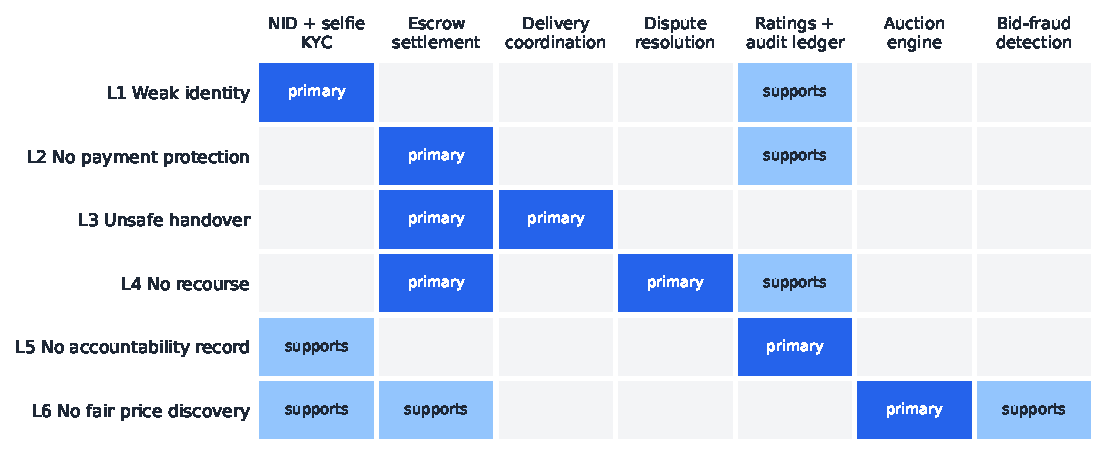
\includegraphics[width=\textwidth]{fig13_mapping.pdf}
  \caption{Which TrustBazaar feature addresses which Bikroy loophole. Dark cells: the feature is
  the primary fix; light cells: it supports the fix. Escrow settlement is the primary fix for
  three loopholes. Mapping derived from the TrustBazaar proposal~\cite{proposal}.}
  \label{fig:mapping}
\end{figure}

\subsection{Same transaction, different control}

Figure~\ref{fig:lifecycle} traced a used-goods deal through six stages and showed that Bikroy
has no control over the last three. Figure~\ref{fig:lifecycle_tb} draws the same six stages for
TrustBazaar. The difference is concentrated in the stages where the documented scams happen:
payment, handover and dispute.

\begin{figure}[H]
  \centering
  \resizebox{\textwidth}{!}{% Same six stages as Figure 11: Bikroy (top row) vs TrustBazaar (bottom row)
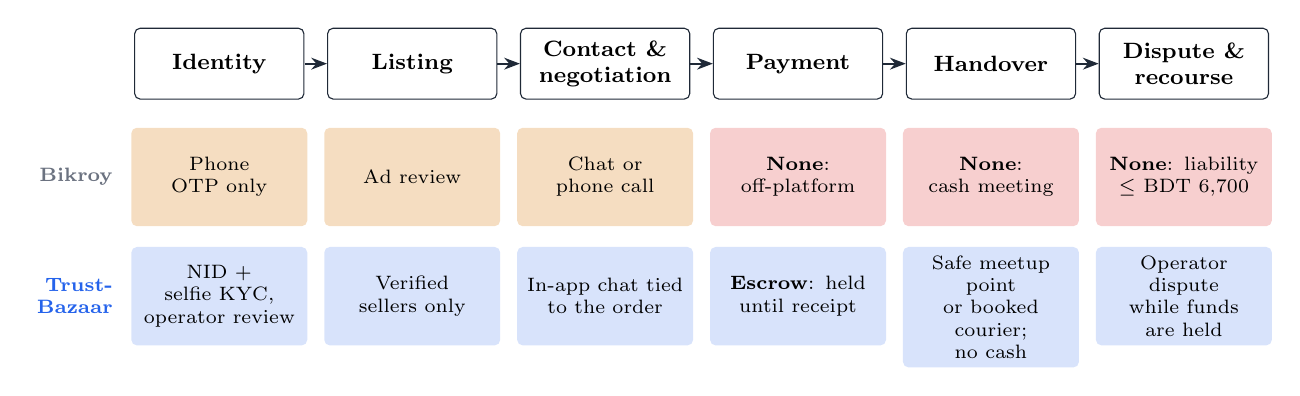
\begin{tikzpicture}[
  font=\footnotesize,
  stage/.style={draw=ink, fill=white, rounded corners=2pt, minimum width=2.15cm,
                minimum height=0.9cm, align=center, font=\footnotesize\bfseries},
  cover/.style={rounded corners=2pt, minimum width=2.15cm, minimum height=1.25cm,
                align=center, text width=2.0cm, font=\scriptsize},
  flow/.style={-{Stealth[length=2mm]}, draw=ink, thick}]

  \foreach \i/\name in {1/Identity, 2/Listing, 3/Contact \&\\negotiation,
                        4/Payment, 5/Handover, 6/Dispute \&\\recourse}{
    \node[stage] (s\i) at ({(\i-1)*2.45},0) {\name};
  }
  \foreach \a/\b in {1/2,2/3,3/4,4/5,5/6}{ \draw[flow] (s\a) -- (s\b); }

  % Bikroy row
  \node[cover, fill=partial!25] (b1) [below=0.35cm of s1] {Phone OTP only};
  \node[cover, fill=partial!25] (b2) [below=0.35cm of s2] {Ad review};
  \node[cover, fill=partial!25] (b3) [below=0.35cm of s3] {Chat or phone call};
  \node[cover, fill=bad!22]     (b4) [below=0.35cm of s4] {\textbf{None}:\\off-platform};
  \node[cover, fill=bad!22]     (b5) [below=0.35cm of s5] {\textbf{None}:\\cash meeting};
  \node[cover, fill=bad!22]     (b6) [below=0.35cm of s6] {\textbf{None}: liability\\$\le$ BDT 6,700};

  % TrustBazaar row
  \node[cover, fill=good!18] (t1) [below=0.25cm of b1] {NID + selfie KYC,\\operator review};
  \node[cover, fill=good!18] (t2) [below=0.25cm of b2] {Verified sellers only};
  \node[cover, fill=good!18] (t3) [below=0.25cm of b3] {In-app chat tied\\to the order};
  \node[cover, fill=good!18] (t4) [below=0.25cm of b4] {\textbf{Escrow}: held\\until receipt};
  \node[cover, fill=good!18] (t5) [below=0.25cm of b5] {Safe meetup point\\or booked courier;\\no cash};
  \node[cover, fill=good!18] (t6) [below=0.25cm of b6] {Operator dispute\\while funds\\are held};

  \node[anchor=east, font=\scriptsize\bfseries, text=muted, align=right]
    at ([xshift=-3pt]b1.west) {Bikroy};
  \node[anchor=east, font=\scriptsize\bfseries, text=good, align=right]
    at ([xshift=-3pt]t1.west) {Trust-\\Bazaar};
\end{tikzpicture}
}
  \caption{The six stages of a used-goods transaction, comparing Bikroy's control (top row,
  from Figure~\ref{fig:lifecycle}) with TrustBazaar's design (bottom row). Sources: Bikroy
  \cite{fs_fraud,ds_jiji,bikroy_terms}; TrustBazaar~\cite{proposal}.}
  \label{fig:lifecycle_tb}
\end{figure}

The core of this design is the escrow state machine in Figure~\ref{fig:escrow_states}. It
implements the proposal's third acceptance criterion: an escrow payment is never released
to a seller without either the buyer's explicit confirmation or a genuine timeout. It also
implements the fourth: a payment notice (webhook) that the provider delivers twice is never
processed twice~\cite{proposal}. Because the money is still held when a dispute is raised, a
refund is a database operation, not a police case.

\begin{figure}[H]
  \centering
  \resizebox{0.95\textwidth}{!}{% Escrow settlement state machine (TrustBazaar proposal, Objective 3 and Acceptance criterion 3)
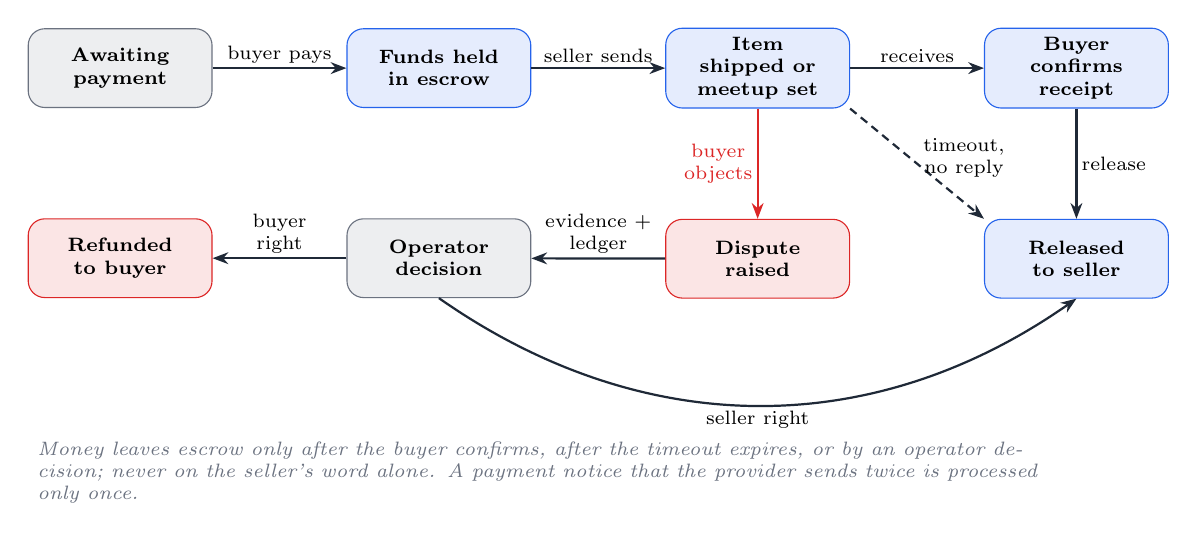
\begin{tikzpicture}[
  font=\footnotesize, node distance=14mm and 17mm,
  st/.style={draw=#1, fill=#1!12, rounded corners=6pt, minimum height=1.0cm,
             text width=2.1cm, align=center, font=\scriptsize\bfseries},
  tr/.style={-{Stealth[length=2mm]}, thick, draw=ink},
  lab/.style={font=\scriptsize, inner sep=1.5pt, align=center}]

  \node[st=muted]                 (pay)  {Awaiting\\payment};
  \node[st=good, right=of pay]    (held) {Funds held\\in escrow};
  \node[st=good, right=of held]   (ship) {Item shipped or\\meetup set};
  \node[st=good, right=of ship]   (conf) {Buyer confirms\\receipt};
  \node[st=good, below=of conf]   (rel)  {Released\\to seller};
  \node[st=bad, below=of ship]    (disp) {Dispute\\raised};
  \node[st=muted, below=of held]  (dec)  {Operator\\decision};
  \node[st=bad, below=of pay]     (ref)  {Refunded\\to buyer};

  \draw[tr] (pay) -- node[lab, above]{buyer pays} (held);
  \draw[tr] (held) -- node[lab, above]{seller sends} (ship);
  \draw[tr] (ship) -- node[lab, above]{receives} (conf);
  \draw[tr] (conf) -- node[lab, right]{release} (rel);
  \draw[tr, densely dashed] (ship.south east) -- (rel.north west)
     node[lab, pos=0.45, right=1mm]{timeout,\\no reply};
  \draw[tr, bad] (ship) -- node[lab, left, text=bad]{buyer\\objects} (disp);
  \draw[tr] (disp) -- node[lab, above]{evidence +\\ledger} (dec);
  \draw[tr] (dec) -- node[lab, above]{buyer\\right} (ref);
  \draw[tr] (dec.south) to[out=-35, in=-145] node[lab, below, pos=0.5]{seller right} (rel.south);

  \node[font=\scriptsize\itshape, text=muted, align=left, anchor=north west, text width=13cm]
    at ([yshift=-17mm]ref.south west)
    {Money leaves escrow only after the buyer confirms, after the timeout expires, or by an
     operator decision; never on the seller's word alone. A payment notice that the provider
     sends twice is processed only once.};
\end{tikzpicture}
}
  \caption{TrustBazaar's escrow settlement as a state machine. Money can leave escrow by only
  three routes: buyer confirmation, an expired timeout, or an operator's dispute decision.
  Based on Objective~3 and Acceptance criteria~3--4 of the proposal~\cite{proposal}.}
  \label{fig:escrow_states}
\end{figure}

\subsection{Replaying the documented scams}

Table~\ref{tab:replay} takes each scam pattern documented in Section~\ref{sec:users}
(Table~\ref{tab:scams}) and shows where TrustBazaar's design stops it.

\begin{table}[H]
  \centering
  \small
  \caption{The scam patterns documented on Bikroy, replayed against TrustBazaar's design.}
  \label{tab:replay}
  \begin{tabularx}{\textwidth}{@{}>{\raggedright\arraybackslash}p{4.0cm} Y@{}}
    \toprule
    \textbf{Documented scam} & \textbf{What happens on TrustBazaar} \\
    \midrule
    Fake seller, advance payment (Muktagacha)~\cite{ds_muktagacha}
      & Each SIM-bought account would still need a real NID and selfie to list, blocking the
        scam at the start. Even if a fake listing slipped through, the buyer's money sits in
        escrow, so non-delivery leads to a refund instead of a loss. \\
    \addlinespace
    Lure and robbery (2014)~\cite{dt_2014}
      & The system suggests a public meetup point, or the buyer uses a courier and never meets
        the seller. Both parties' verified identities are on record. \\
    \addlinespace
    Counterfeit or swapped cash (2023 iPhone case)~\cite{pa_2023}
      & No cash at the meeting: payment is already held in escrow. \\
    \addlinespace
    Fake or replica goods~\cite{fs_fraud}
      & The buyer inspects the item and can raise a dispute before any money is released. \\
    \addlinespace
    Fake inquiries after paid promotion~\cite{trustpilot}
      & TrustBazaar's revenue is a commission on \emph{completed} sales~\cite{proposal}, not a
        charge per click. The platform earns only when a real deal happens, unlike the
        pay-per-click model Bikroy is moving to under Jiji~\cite{fs_jiji}. \\
    \bottomrule
  \end{tabularx}
\end{table}

\subsection{Market position: what TrustBazaar offers that incumbents do not}

The mapping above implies five points about where TrustBazaar sits in the market.

\begin{enumerate}[label=\textbf{\arabic*.}]
  \item \textbf{It targets a slice of the market, not the whole of it.} Most of Bikroy's transaction value is in
  cars and property~\cite{fs_jiji}, but most of its ads are used phones, electronics and
  household goods (Section~\ref{sec:catalogue}). TrustBazaar is designed for that
  individual-to-individual resale of used goods~\cite{proposal}, the part of the market where
  the documented scams cluster~\cite{ds_muktagacha,pa_2023} and where a buyer has no way to
  verify a stranger.

  \item \textbf{It differs in kind from every previous challenger.} OLX, Ekhanei and Jiji all ran
  listing boards~\cite{fs_ekhanei,intellinews}. None of them competed on the transaction
  itself. TrustBazaar is a different kind of product: a settlement platform, not a
  classifieds board.

  \item \textbf{It applies a protection Bangladesh has already adopted.} After the Evaly failures, the
  state required escrow for e-commerce payments~\cite{tbs_escrow}, and money still held in
  escrow was returned to buyers~\cite{fe_refund}. That regime never reached person-to-person
  resale (Section~\ref{sec:users}). TrustBazaar applies a protection the state has already
  validated to the part of the market it misses.

  \item \textbf{It suits the individual sellers Bikroy is moving away from.} Under Jiji, pay-per-click
  bidding favours sellers with marketing budgets~\cite{fs_jiji}. A fee charged only on completed
  deals better suits someone selling one used phone.

  \item \textbf{It offers what Facebook groups do not.} They have no verification, no payment handling
  and no record of who committed to buy~\cite{proposal}. For a buyer about to send a large sum to a
  stranger, TrustBazaar's offer is simple: the money does not move until the buyer has
  the item.
\end{enumerate}

\subsection{Limits and risks}

The design does not remove every barrier to adoption. Table~\ref{tab:limits} lists the main
risks and how TrustBazaar's design responds to each.

\begin{table}[H]
  \centering
  \small
  \caption{Main risks to TrustBazaar's adoption and the design response.}
  \label{tab:limits}
  \begin{tabularx}{\textwidth}{@{}>{\raggedright\arraybackslash}p{2.4cm}
                                  >{\raggedright\arraybackslash}p{4.6cm} Y@{}}
    \toprule
    \textbf{Risk} & \textbf{Why it is real} & \textbf{Design response} \\
    \midrule
    Network effect
      & Bikroy has about 400{,}000 monthly buyers and 100{,}000 monthly sellers~\cite{fs_jiji};
        a new platform starts with none.
      & This is the main open risk and is not solved by design alone. The project's aim is to
        demonstrate that the trust mechanisms work correctly, not to reach market
        scale~\cite{proposal}. \\
    \addlinespace
    KYC friction
      & Users already complain about Bikroy's manual checks~\cite{trustpilot}.
      & KYC is done once, not per ad. It gives the user something back (escrow protection and
        a verified badge) rather than being a cost with no return. \\
    \addlinespace
    Seller cash-flow delay
      & Escrow holds the money until the buyer confirms.
      & An automatic release timeout means a silent buyer cannot hold the funds
        indefinitely~\cite{proposal}. \\
    \addlinespace
    Regulation
      & Holding customers' money requires a licensed payment partner.
      & The academic build uses sandbox and test-mode integrations, stated openly~\cite{proposal}.
        A real launch would route funds through a licensed gateway's escrow service, the model
        the 2021 Bangladesh Bank rule uses~\cite{tbs_escrow}. \\
    \addlinespace
    Fees
      & Buyers and sellers may resist paying a commission.
      & The fee is charged only on a successful, protected deal, set against the documented
        cost of being scammed. \\
    \bottomrule
  \end{tabularx}
\end{table}

\subsection{Summary}

Bikroy has led the market since 2012 without being challenged on what it does not do. It
is a listing board that leaves payment, handover and disputes to chance, and its own terms say
so~\cite{bikroy_terms}. TrustBazaar does not compete on the number of ads. It closes the six
loopholes that Bikroy, Facebook groups and the 2021 escrow rule all leave open for individual
resale. Its value proposition is therefore not scale but safety: it is designed to protect
exactly the deals that Bikroy's terms decline responsibility for.

\section{The Competitive Landscape: Why No Existing Platform Fills the Gap}
\label{sec:landscape}

Sections~\ref{sec:history}--\ref{sec:solution} compared TrustBazaar with Bikroy. Bikroy is not the only
option, however: Facebook and Daraz also carry resale and online sales. This section compares
TrustBazaar with every realistic alternative available to a Bangladeshi reselling a used item
today, including digital items such as game accounts and event tickets, and shows that the
combination TrustBazaar offers does not exist in the market.

\subsection{Bikroy under Jiji}

Since May 2026 Bikroy runs on Jiji's platform~\cite{fs_jiji}. Jiji's safety model is the same
as Bikroy's: it moderates ads before publication, uses automated fraud detection, and instructs
buyers never to pay before receiving an item, but it does not hold the payment
itself~\cite{jiji_kenya}. The acquisition gave Bikroy a new owner, not a new trust model.

\subsection{Facebook Marketplace and buy-and-sell groups}
\label{sec:facebook}

Facebook Marketplace has launched in Bangladesh, but Facebook does not facilitate payment or
delivery for person-to-person Marketplace sales, and as of 2021 its Shops checkout was not
available in Bangladesh~\cite{fs_facebook}. Buyers and sellers therefore settle outside the
platform, exactly as on Bikroy.

Scams on Facebook follow the same advance-payment pattern documented in
Section~\ref{sec:users}. In February 2021, Dhaka police arrested five members of a gang that
advertised goods on a Facebook page, took 50\% advance payments plus delivery charges, and then
shut down both the page and the mobile-banking account. The gang had been operating for about
six months and had opened its accounts using \emph{fake national identity documents}, which
made it hard to trace~\cite{tbs_fcommerce}. This last detail matters for TrustBazaar and is
discussed in Section~\ref{sec:threats}.

\subsubsection*{Digital goods: game accounts, tickets and the ``admin deal''}

Facebook buy-and-sell groups are also used to trade \emph{digital} goods: accounts for games
such as PUBG Mobile, Free Fire and Clash of Clans, Steam or Epic Games accounts, and event
tickets. These items cannot be inspected like a phone. In the groups our team is familiar with,
the usual way to manage the risk is an ``admin deal'', in which the group's admin acts as a
middleman: the buyer sends the money to the admin, the seller
sends the account ID and password to the admin, and the admin passes each on
(Figure~\ref{fig:admin_deal}). We did not find a published study measuring how often these
deals fail, but the available evidence shows why the structure itself is unsafe.

\begin{figure}[H]
  \centering
  \resizebox{0.97\textwidth}{!}{% The Facebook-group "admin deal" for digital goods, and its failure modes
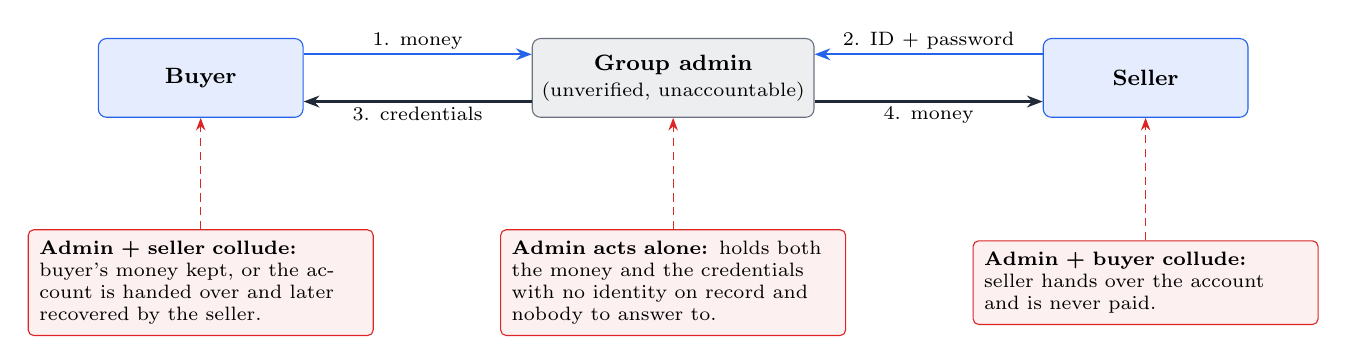
\begin{tikzpicture}[
  font=\footnotesize,
  party/.style={draw=#1, fill=#1!12, rounded corners=3pt, minimum width=2.6cm,
                minimum height=1.0cm, align=center, font=\footnotesize\bfseries},
  tr/.style={-{Stealth[length=2mm]}, thick, draw=#1},
  lab/.style={font=\scriptsize, fill=white, inner sep=1.5pt, align=center},
  fail/.style={draw=bad, fill=bad!7, rounded corners=2pt, text width=4.1cm,
               align=left, font=\scriptsize, inner sep=4pt}]

  \node[party=good]  (B) at (0,0)    {Buyer};
  \node[party=muted] (A) at (6,0)    {Group admin\\{\scriptsize\normalfont (unverified, unaccountable)}};
  \node[party=good]  (S) at (12,0)   {Seller};

  \draw[tr=good] ([yshift=3mm]B.east) -- node[lab, above]{1. money} ([yshift=3mm]A.west);
  \draw[tr=good] ([yshift=3mm]S.west) -- node[lab, above]{2. ID + password} ([yshift=3mm]A.east);
  \draw[tr=ink]  ([yshift=-3mm]A.west) -- node[lab, below]{3. credentials} ([yshift=-3mm]B.east);
  \draw[tr=ink]  ([yshift=-3mm]A.east) -- node[lab, below]{4. money} ([yshift=-3mm]S.west);

  \node[fail] (f1) at (0,-2.6)
    {\textbf{Admin + seller collude:} buyer's money kept, or the account is handed over
     and later recovered by the seller.};
  \node[fail] (f2) at (6,-2.6)
    {\textbf{Admin acts alone:} holds both the money and the credentials with no identity
     on record and nobody to answer to.};
  \node[fail] (f3) at (12,-2.6)
    {\textbf{Admin + buyer collude:} seller hands over the account and is never paid.};

  \draw[-{Stealth[length=1.6mm]}, bad, densely dashed] (f1.north) -- (B.south);
  \draw[-{Stealth[length=1.6mm]}, bad, densely dashed] (f2.north) -- (A.south);
  \draw[-{Stealth[length=1.6mm]}, bad, densely dashed] (f3.north) -- (S.south);
\end{tikzpicture}
}
  \caption{The Facebook-group ``admin deal'' for digital goods. A single unverified person holds
  both the money and the credentials, which allows three kinds of fraud. Risks of account
  transfer as described by Supercell~\cite{supercell_fairplay}; admin misconduct illustrated by
  the 2026 BCEC case~\cite{fe_bcec}.}
  \label{fig:admin_deal}
\end{figure}

\begin{itemize}
  \item \textbf{Admins hold power without accountability.} In July 2026 the Criminal
  Investigation Department (CID) arrested the 21-year-old admin of the Facebook group
  ``Bangladesh Concert \& Event Connects''. He had approved posts selling tickets for an
  Atif Aslam concert that used images of tickets from a previously cancelled concert, and when
  the organisers asked him to remove them, he demanded Tk~1~lakh instead. A case was filed under
  the Cyber Security Act at Paltan Police Station~\cite{fe_bcec}. The person members trusted to
  keep the group safe was the one exploiting it.

  \item \textbf{The game companies themselves name the risks.} Supercell's policy lists the
  dangers of buying an account: the seller may never deliver it, the same account may be sold
  to several buyers, and the original owner may keep access and take it back. Supercell also
  permanently bans accounts confirmed to have changed hands~\cite{supercell_fairplay}.

  \item \textbf{Account sales break the publishers' terms.} Steam's Subscriber Agreement forbids
  sharing a password or letting others use an account, and does not allow accounts to be sold or
  transferred (Section~1.C)~\cite{steam_ssa}. Garena's terms for Free Fire make accounts
  non-transferable and for personal use only (Section~6.2)~\cite{sk_garena}. A buyer can
  therefore lose a purchased account to a ban even if the seller is honest.

  \item \textbf{The same fraud appears in the region.} In September 2022 Pakistan's Federal
  Investigation Agency arrested suspects in Faisalabad for selling fake PUBG accounts; one
  complainant alone had lost about PKR~820{,}000~\cite{techjuice_pubg}.

  \item \textbf{Bikroy offers no answer either.} Bikroy hosts game-account listings, for example
  a Free Fire account advertised for BDT~9{,}500 in 2020, but shows the same safety tips it uses for
  physical goods: meet in a safe public place and inspect the item before
  paying~\cite{bikroy_ff}. That advice cannot be followed for a password.

  \item \textbf{Large platforms have recognised the problem.} In July 2025 Steam introduced a
  seven-day trade-protection window during which item trades can be reversed, specifically to
  counter scams and compromised accounts~\cite{pcworld_steam}. The industry's own answer to
  digital-goods fraud is a holding period, the same principle as escrow.
\end{itemize}

Digital goods therefore combine every weakness identified in this report. There is nothing to
inspect, identities are unverified, the money moves first, and the only safeguard is a single
unaccountable middleman. The revised TrustBazaar proposal therefore adds a dedicated
game-account escrow, in which ownership is verified before listing, credentials are encrypted
so that only the buyer can read them, and payment is held through a protection period after
takeover~\cite{proposal_rev}. Because account trading conflicts with the publishers' terms, the
proposal discloses that risk to buyers before payment rather than presenting these sales as
approved by the publisher.

\subsection{Daraz}

Daraz does protect buyers. Since October 2025 it has offered a 14-day return window on
applicable items, with free pickup or drop-off and refunds that include delivery
charges~\cite{pa_daraz}. However, Daraz is built for businesses selling new stock: according to
our proposal's market review, its seller requirements are built around business registration
rather than personal identity checks, and it offers no auction format~\cite{proposal}. It is not
designed for one person selling one used item to another.

\subsection{Side-by-side comparison}

Table~\ref{tab:landscape} and Figure~\ref{fig:capabilities} compare the four platforms on the
capabilities this report has shown to matter.

\begin{table}[H]
  \centering
  \small
  \caption{Capabilities of the main platforms available for resale in Bangladesh.}
  \label{tab:landscape}
  \begin{tabularx}{\textwidth}{@{}>{\raggedright\arraybackslash}p{2.6cm}
     >{\raggedright\arraybackslash}X >{\raggedright\arraybackslash}X
     >{\raggedright\arraybackslash}X >{\raggedright\arraybackslash}X@{}}
    \toprule
    \textbf{Capability} & \textbf{Bikroy / Jiji} & \textbf{Facebook} & \textbf{Daraz} &
      \textbf{TrustBazaar} \\
    \midrule
    Built for individuals' used goods & Yes & Yes & No: businesses, new stock~\cite{proposal}
      & Yes \\
    Identity verification & Phone OTP~\cite{fs_fraud} & Facebook account only;
      fake NIDs used~\cite{tbs_fcommerce} & Business registration~\cite{proposal}
      & NID + selfie KYC \\
    Who holds the payment & Nobody~\cite{bikroy_terms,jiji_kenya} & Nobody~\cite{fs_facebook}
      & Platform checkout & Escrow until receipt \\
    Refund if item is bad or missing & No; liability $\le$ BDT~6{,}700~\cite{bikroy_terms}
      & No & Yes, 14-day returns~\cite{pa_daraz} & Yes, dispute while funds are held \\
    Handover & Meet in person~\cite{bikroy_safety} & Arranged by users
      & Platform logistics~\cite{pa_daraz} & Safe meetup point or booked courier \\
    Dispute process & None~\cite{bikroy_terms} & Group admin at best~\cite{fe_bcec}
      & Returns process & Operator decision using ledger \\
    Fair auction & No & Informal comment bidding~\cite{proposal} & No~\cite{proposal}
      & Server-timed, anti-sniping \\
    Digital goods & Listed with physical-goods advice~\cite{bikroy_ff} & Admin deals
      & Not examined & Game-account escrow~\cite{proposal_rev} \\
    \bottomrule
  \end{tabularx}
\end{table}

\begin{figure}[H]
  \centering
  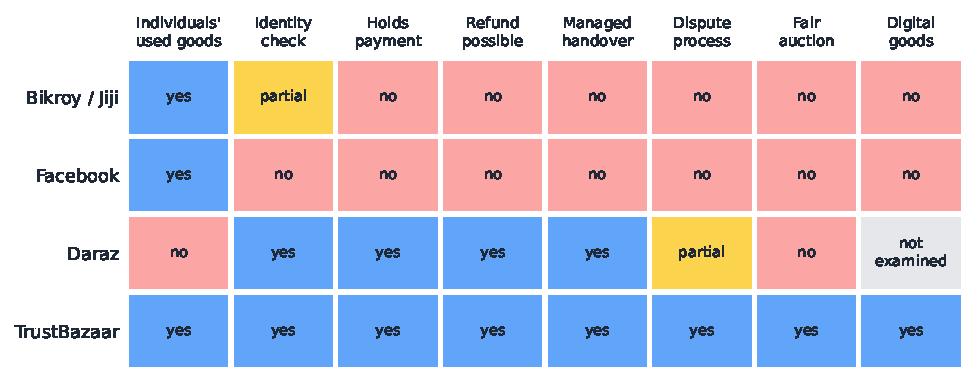
\includegraphics[width=\textwidth]{fig16_capabilities.pdf}
  \caption{Capability matrix of Table~\ref{tab:landscape}. Blue: yes; yellow: partial; red: no;
  grey: not examined. Daraz's identity and auction entries come from
  our proposal's market review~\cite{proposal}; all other sources are given in
  Table~\ref{tab:landscape}.}
  \label{fig:capabilities}
\end{figure}

\subsection{The empty quadrant}

Two questions separate the platforms: \emph{who is it built for} (individuals selling used goods,
or businesses selling new stock), and \emph{does the platform protect the transaction} (hold the
money, offer refunds, resolve disputes)? Bikroy and Facebook are built for individuals but
protect nothing. Daraz protects the transaction but is built for businesses. No existing
platform does both (Figure~\ref{fig:positioning}).

\begin{figure}[H]
  \centering
  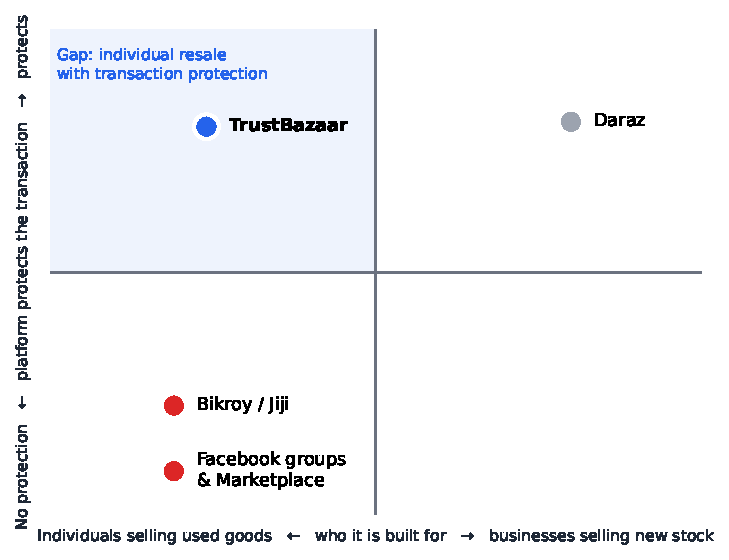
\includegraphics[width=0.72\textwidth]{fig17_positioning.pdf}
  \caption{Qualitative positioning of the platforms, based on the capabilities in
  Table~\ref{tab:landscape}. Positions show which quadrant each platform belongs to, not a
  measured score.}
  \label{fig:positioning}
\end{figure}

Each existing platform proves half of TrustBazaar's case. Bikroy and Facebook prove the
\emph{demand}: hundreds of thousands of individuals resell used goods online every
month~\cite{fs_jiji}. Daraz and the 2021 escrow rule prove that the \emph{protection} works and
that Bangladeshi buyers accept platform-managed payments and returns~\cite{pa_daraz,tbs_escrow}.
TrustBazaar combines the two.

\subsection{Threats and honest limits}
\label{sec:threats}

\begin{table}[H]
  \centering
  \small
  \caption{Competitive threats and our assessment.}
  \label{tab:threats}
  \begin{tabularx}{\textwidth}{@{}>{\raggedright\arraybackslash}p{3.6cm} Y@{}}
    \toprule
    \textbf{Threat} & \textbf{Assessment} \\
    \midrule
    Fake NIDs can defeat KYC, as the 2021 Facebook gang showed~\cite{tbs_fcommerce}
      & KYC raises the cost of fraud; it does not eliminate it. TrustBazaar adds a selfie match and
        operator review~\cite{proposal}. More importantly, escrow means a fake identity still
        cannot take the buyer's money: payment is released only when the buyer confirms
        receipt. Identity checks and escrow cover each other's gaps. \\
    \addlinespace
    Daraz could open to individuals' used goods
      & Possible. If it did, that would confirm the gap is real; TrustBazaar's auction and
        person-to-person delivery design would still differ from Daraz's business model. \\
    \addlinespace
    Jiji could add escrow to Bikroy
      & Also possible. So far Jiji's stated model is pay-on-delivery advice, not held
        payments~\cite{jiji_kenya}. \\
    \addlinespace
    Facebook's reach
      & Facebook's user base cannot be matched. TrustBazaar's case is not reach but the one thing
        Facebook does not offer for person-to-person deals in Bangladesh: holding the
        money~\cite{fs_facebook}. \\
    \bottomrule
  \end{tabularx}
\end{table}

TrustBazaar's advantage is its design, not a barrier competitors cannot copy. The project's aim is to
show that this design can be built correctly,
with concurrency-safe auctions and escrow that never releases money wrongly~\cite{proposal},
not to claim that incumbents can never follow.

\subsection{Summary}

Every platform available to a Bangladeshi reseller today fails on at least one of two counts.
Bikroy, Jiji and Facebook serve individuals but leave the transaction to chance, and for digital
goods they leave it to an unaccountable group admin. Daraz protects the transaction but is not
built for individuals reselling used goods. TrustBazaar is designed to combine both. Its case for adoption
rests not on the other platforms being poor at what they do, but on none of them doing this.

\section{Conclusions: Why Users Would Move to TrustBazaar}
\label{sec:conclusion}

This section draws together the findings of
Sections~\ref{sec:history}--\ref{sec:landscape}. Taken together, they show that Bikroy and
Facebook Marketplace succeed at \emph{connecting} buyers and sellers, but that neither protects
the \emph{transaction} that follows. Section~\ref{sec:history} showed that this weakness has
existed since Bikroy began; Section~\ref{sec:users} showed where it harms users;
Section~\ref{sec:solution} showed how TrustBazaar's design addresses each gap; and
Section~\ref{sec:landscape} showed that no other platform addresses them.

\subsection{Key findings and their implications for adoption}

\paragraph{Finding 1: Bikroy's trust problem was managed, never solved.}
Bikroy's own 2014 audit found that one ad in three was not genuine (Figure~\ref{fig:genuine}).
Every measure it took afterwards cleaned up listings but neither protected a transaction nor
helped a victim recover a loss (Table~\ref{tab:response}), and the audit was never repeated
publicly. Users have therefore lived with the same risk for over a decade. TrustBazaar is
designed to remove that risk rather than warn about it (Table~\ref{tab:mapping}).

\paragraph{Finding 2: Bikroy is losing position and changing in ways that disadvantage
individual sellers.}
Bikroy fell from the 8th largest local website in 2014 to between \#67 and \#104 in 2026
(Figure~\ref{fig:rank}), with month-on-month traffic declines (Figure~\ref{fig:traffic}). Its
parent company stopped investing after 2015 and sold it to Jiji in 2026
(Figure~\ref{fig:saltside}, Section~\ref{sec:sale}), and it is moving to pay-per-click pricing
that favours sellers with marketing budgets (Section~\ref{sec:downfall}). TrustBazaar charges a
commission only on completed deals (Table~\ref{tab:replay}), a better fit for the individual
seller Bikroy is moving away from.

\paragraph{Finding 3: users like the app but are not protected by it.}
The Bikroy app is well rated (Figure~\ref{fig:ratings}), but app ratings measure usability, not
safety. Among surveyed cybercrime victims, 40\% lost money and only 12\% took legal action
(Figure~\ref{fig:ccaf}), so most fraud is never recorded. This explains how users can keep using
Bikroy while remaining exposed. TrustBazaar does not require them to give up a familiar tool; it
offers the protection that tool lacks.

\paragraph{Finding 4: every documented scam occurs where Bikroy has no control.}
The scam patterns in Table~\ref{tab:scams} strike at payment, handover and dispute, the three
stages Bikroy does not control (Figure~\ref{fig:lifecycle}). Both the advance-payment scam
(Figure~\ref{fig:advance}) and the cash note-swap scam (Figure~\ref{fig:noteswap}) depend on
money changing hands outside the platform. Replayed against TrustBazaar, each pattern is stopped
by escrow, verified identity or managed delivery (Table~\ref{tab:replay}), and all six stages of
a deal come under platform control (Figure~\ref{fig:lifecycle_tb}).

\paragraph{Finding 5: escrow already works in Bangladesh, but not for person-to-person deals.}
Bangladesh Bank made escrow mandatory for e-commerce in 2021, and money still held in escrow
could be returned to buyers (Figure~\ref{fig:escrow}). That rule never reached classifieds,
because payment on Bikroy never passes through the platform (Section~\ref{sec:escrowlesson}).
TrustBazaar's escrow settlement (Figure~\ref{fig:escrow_states}) extends a protection the country
has already adopted to the gap left open by loophole L2 (Section~\ref{sec:loopholes}).

\paragraph{Finding 6: Facebook is no safer, and its group admins are a risk of their own.}
Facebook does not handle payment for person-to-person sales in Bangladesh, and scams there follow
the same advance-payment pattern, including accounts opened with fake national IDs
(Section~\ref{sec:facebook}). For digital goods, users rely on group admins who hold both the
money and the credentials (Figure~\ref{fig:admin_deal}), a structure shown to be open to abuse by
the 2026 arrest of a group admin. TrustBazaar replaces the trusted individual with a system that
holds the money and records every decision (Table~\ref{tab:mapping}, loophole L5).

\paragraph{Finding 7: no existing platform combines individual resale with transaction
protection.}
Bikroy and Facebook serve individuals but protect nothing; Daraz protects transactions but serves
businesses selling new stock (Table~\ref{tab:landscape}, Figure~\ref{fig:capabilities}). The
quadrant for individual resale with transaction protection is empty
(Figure~\ref{fig:positioning}). TrustBazaar is designed for that quadrant, and escrow alone is the
primary fix for three of the six loopholes (Figure~\ref{fig:mapping}).

\subsection{Summary of adoption drivers}

Table~\ref{tab:drivers} condenses these findings into the reasons a user would choose
TrustBazaar, each linked to the evidence in this report.

\begin{table}[!htbp]
  \centering
  \small
  \caption{Adoption drivers: what users face on existing platforms, where this report shows it,
  and what TrustBazaar offers instead.}
  \label{tab:drivers}
  \begin{tabularx}{\textwidth}{@{}>{\raggedright\arraybackslash}p{4.2cm}
                                  >{\raggedright\arraybackslash}p{3.3cm} Y@{}}
    \toprule
    \textbf{What users face today} & \textbf{Shown in} & \textbf{What TrustBazaar offers} \\
    \midrule
    Payment goes straight to a stranger; no platform holds it
      & Fig.~\ref{fig:lifecycle}, Table~\ref{tab:landscape}
      & Escrow: seller paid only after the buyer confirms receipt \\
    \addlinespace
    Robbery and counterfeit cash at meetups
      & Table~\ref{tab:scams}, Fig.~\ref{fig:noteswap}
      & No cash at the meeting; safe meetup point or booked courier \\
    \addlinespace
    Identity is a phone number or a fake NID
      & Fig.~\ref{fig:advance}, Sec.~\ref{sec:facebook}
      & NID + selfie KYC, backed by escrow \\
    \addlinespace
    No refund or help after a scam
      & Table~\ref{tab:response}, Fig.~\ref{fig:ccaf}
      & Dispute raised while the money is still held \\
    \addlinespace
    Group admins hold money and passwords unchecked
      & Fig.~\ref{fig:admin_deal}
      & The system, not a person, holds the money; decisions logged \\
    \addlinespace
    Pay-per-click pricing favours bigger sellers
      & Sec.~\ref{sec:sale}, Sec.~\ref{sec:downfall}
      & Commission only on completed deals \\
    \addlinespace
    No fair auction format
      & Table~\ref{tab:landscape}
      & Server-timed auction with anti-sniping \\
    \bottomrule
  \end{tabularx}
\end{table}

\subsection{Likely order of adoption}

Comparing where the documented scams cluster (Table~\ref{tab:scams}) with what TrustBazaar
addresses (Table~\ref{tab:mapping}) suggests the order in which users are most likely to adopt
it:

\begin{enumerate}[label=\textbf{\arabic*.}]
  \item \textbf{Buyers of mid- and high-value used electronics.} The advance-payment and
  note-swap scams in Figures~\ref{fig:advance} and~\ref{fig:noteswap} involved phones and
  electronics, where losing the money is most costly.
  \item \textbf{Individual sellers.} They are exposed to fake buyers (Figure~\ref{fig:noteswap})
  and to Bikroy's new pricing (Finding~2). Escrow protects them too: payment is secured before
  the item leaves their hands (Figure~\ref{fig:escrow_states}).
  \item \textbf{Sellers seeking competitive bidding.} Neither Bikroy nor Facebook offers a fair
  auction (loophole L6, Table~\ref{tab:landscape}).
  \item \textbf{Game-account buyers and sellers.} They currently depend on unaccountable group
  admins (Figure~\ref{fig:admin_deal}); the game-account escrow in the revised
  proposal~\cite{proposal_rev} replaces that middleman, although publisher bans remain a risk the
  platform can disclose but not prevent (Section~\ref{sec:facebook}).
\end{enumerate}

\subsection{Limitations of this analysis}

The conclusions above should be read within the following limits:

\begin{itemize}
  \item \textbf{Incumbents retain scale.} Bikroy still reports about 400{,}000 monthly buyers
  (Section~\ref{sec:present}), and Facebook's reach cannot be matched (Table~\ref{tab:threats}).
  Users will keep browsing there. The realistic shift is per transaction, not total: users are
  likely to move the risky step, paying a stranger, to where the money is protected
  (Tables~\ref{tab:limits} and~\ref{tab:threats}).
  \item \textbf{Fraud is reduced, not eliminated.} KYC can be defeated by fake national IDs
  (Section~\ref{sec:facebook}); TrustBazaar's response is that escrow and identity checks cover
  each other's gaps (Table~\ref{tab:threats}).
  \item \textbf{Evidence gaps.} The most recent police case naming Bikroy dates from 2023
  (Section~\ref{sec:still}); traffic figures are third-party estimates (Table~\ref{tab:then_now});
  the Trustpilot sample is small (Figure~\ref{fig:ratings}); and the description of admin deals
  rests on the authors' familiarity with these groups (Section~\ref{sec:facebook}).
  \item \textbf{No primary user data.} This analysis uses published sources only. A survey of
  buyers and sellers would be needed to measure demand directly.
\end{itemize}

\subsection{Overall conclusion}

Bikroy has led Bangladesh's online classifieds market since 2012, and no challenger has displaced
it, because every challenger competed with the same model: a listing board that connects strangers
and then steps away (Section~\ref{sec:downfall}). The evidence in this report shows that this
model's weakness is structural. Bikroy controls who may post an ad, but not the money, the meeting
or the dispute (Figure~\ref{fig:lifecycle}), and Facebook leaves the same gaps
(Figure~\ref{fig:capabilities}). A new platform therefore does not need more listings than Bikroy
to attract users. It needs to be the place where a buyer's money does not move until the item
arrives, and a seller's item does not leave until the money is secured
(Figure~\ref{fig:escrow_states}). On the evidence gathered here, no existing platform offers this
for person-to-person resale in Bangladesh (Figure~\ref{fig:positioning}), and that is the basis on
which TrustBazaar can persuade users to move.


\begin{thebibliography}{99}
\small

\bibitem{wiki_bikroy} Wikipedia, ``Bikroy.com.''
\url{https://en.wikipedia.org/wiki/Bikroy.com} (accessed 7 Oct 2026).

\bibitem{bn24_2014} Banglanews24, ``32-lakh adverts in Bikroy.com in 2-yr,'' 19 Jun 2014.
\url{https://www.banglanews24.com/english/business/news/bd/23235.details}

\bibitem{fe_2014} J.~U.~Haroon, ``Online mkts expand threefold in a year,''
\emph{The Financial Express}, 29 Sep 2014.
\url{https://today.thefinancialexpress.com.bd/print/online-mkts-expand-threefold-in-a-year}

\bibitem{dt_2014} Dhaka Tribune, ``Beware of fake online advertisements,'' 10 Sep 2014.
\url{https://www.dhakatribune.com/bangladesh/crime/78971/beware-of-fake-online-advertisements}

\bibitem{fs_ekhanei} Future Startup, ``Online classifieds marketplace Ekhanei shuts down,''
16 May 2017.
\url{https://futurestartup.com/2017/05/16/online-classifieds-marketplace-ekhanei-shuts/}

\bibitem{fs_fraud} Future Startup, ``Bikroy takes measures to tackle fraud,'' 25 Feb 2017.
\url{https://futurestartup.com/2017/02/25/bikroy-takes-measures-to-tackle-fraud/}

\bibitem{fs_misha} Future Startup, interview with Misha Ali, Director of Marketing, Bikroy.
\url{https://futurestartup.com/?p=14612}

\bibitem{ds_buynow} The Daily Star, ``Bikroy: More than an online classifieds site,''
interview with Misha Ali. \url{https://www.thedailystar.net/node/1307005}

\bibitem{fs_jiji} Future Startup, ``Jiji acquires Bikroy, Jiji's motivation, Bikroy's
reason, and what it tells about the Bangladesh market,'' 14 May 2026.
\url{https://futurestartup.com/2026/05/14/jiji-acquires-bikroy-jijis-motivation-bikroys-reason-and-what-it-tells-about-the-bangladesh-market/}

\bibitem{intellinews} bne IntelliNews, ``Nigeria's Jiji acquires Bangladeshi classifieds
platform peer Bikroy in first expansion deal outside Africa,'' May 2026.
\url{https://www.intellinews.com/nigeria-s-jiji-acquires-bangladeshi-classifieds-platform-peer-bikroy-in-first-expansion-deal-outside-africa-442571/}

\bibitem{ds_jiji} The Daily Star, ``Nigeria's Jiji acquires Bikroy.com,'' 15 May 2026.
\url{https://thedailystar.net/business/economy/news/nigerias-jiji-acquires-bikroycom-4176081}

\bibitem{similarweb_2026} Similarweb, ``bikroy.com traffic analytics, ranking \& audience
[September 2026].'' \url{https://www.similarweb.com/website/bikroy.com/} (accessed 7 Oct 2026).

\bibitem{semrush_2026} Semrush, ``bikroy.com website traffic, ranking, analytics
[August 2026].'' \url{https://cw.semrush.com/website/bikroy.com/overview/} (accessed 7 Oct 2026).

\bibitem{semrush_2025} Semrush, ``bikroy.com December 2025 traffic stats,'' last updated
13 Jan 2026. \url{https://cw.semrush.com/website/bikroy.com/overview}

\bibitem{trustpilot} Trustpilot, ``Bikroy reviews.''
\url{https://fr-be.trustpilot.com/review/bikroy.com} (accessed 7 Oct 2026).

\bibitem{ds_muktagacha} The Daily Star Bangla, ``Kom dame mobile-er prolobhon diye lakho
taka attmoshat'' [Lakhs of taka embezzled with the lure of cheap mobiles]. Article ID 285801,
\url{https://bangla.thedailystar.net}.

\bibitem{pa_2023} N.~Amin, ``Taka gunte bole koyek second-e manushke boka banan tara''
[They fool people within seconds by asking them to count money], \emph{Prothom Alo},
1 Sep 2023. \url{https://www.prothomalo.com/bangladesh/crime/dmtvv1loj5}

\bibitem{bikroy_terms} Bikroy Marketplace Ltd., ``Terms \& Conditions,'' last updated
17 Apr 2026. \url{https://bikroy.com/rules.html} (accessed 7 Oct 2026).

\bibitem{bikroy_safety} Bikroy.com, ``Safety tips.''
\url{https://bikroy.com/safety-tips.html} (accessed 7 Oct 2026).

\bibitem{bikroy_listing} Bikroy.com, example motorcycle listing showing the platform's
safety tips (2026).
\url{https://bikroy.com/bn/barisal/motorcycles-and-scooters/freedom-runner-2026-eMmVvngxQX2RhG3QQW5xzeKc.html}

\bibitem{proposal} S.~M.~N.~Ahmed, A.~H.~Khan and S.~N.~Sinthia, ``TrustBazaar: A Verified
Peer-to-Peer Auction and Marketplace Platform for Used Goods,'' capstone project proposal,
Department of Software Engineering, Daffodil International University, 30 Sep 2026.

\bibitem{play_store} Google Play, ``Bikroy -- Everything Sells'' (app page and user
reviews), last updated 27 Aug 2026.
\url{https://play.google.com/store/apps/details?id=com.bikroy} (accessed 7 Oct 2026).

\bibitem{ccaf_2024} Cyber Crime Awareness Foundation (CCAF), cybercrime trend report
presented at Independent University, Bangladesh, 29 Jun 2024.
\url{https://iub.ac.bd/news-and-events/news-and-media-archive/2024-July/668621b7b4d241c7517839d0}

\bibitem{itv_hilsa} ITV Bangladesh, ``Onlaine ilish bikrir bigyapon diye protarona korto
tara'' [They cheated people with online ads for hilsa], 21 Aug 2026.
\url{https://www.itvbd.com/country/chittagong/273601}

\bibitem{bdnews_evaly} bdnews24.com (Bangla), Evaly founders sentenced to two years for
fraud, 29 Jan 2025. \url{https://bangla.bdnews24.com/bangladesh/7a6293d95020}

\bibitem{bdnews_eorange} bdnews24.com (Bangla), trial begins in e-Orange fraud case,
16 Feb 2026. \url{https://bangla.bdnews24.com/bangladesh/ede0e11fe3f0}

\bibitem{tbs_escrow} The Business Standard, ``No more direct payments into e-commerce
accounts,'' 25 Aug 2021 (reporting Bangladesh Bank escrow circular of 30 Jun 2021).
\url{https://www.tbsnews.net/economy/no-more-direct-payments-e-commerce-accounts-293197}

\bibitem{fe_refund} The Financial Express, ``Bangladesh government readies repayments to
cheated e-com clients,'' 9 Dec 2021.
\url{https://old.thefinancialexpress.com.bd/trade/bangladesh-government-readies-repayments-to-cheated-e-com-clients-1639020592}

\bibitem{jiji_kenya} TechTrends Kenya, ``Jiji online marketplace Kenya: new security measures
to protect its users,'' 23 Nov 2020.
\url{https://techtrendske.co.ke/2020/11/23/jiji-online-market-place-kenya-new-security-measures-to-protect-its-users-in-a-bid-to-dominate-kenyas-e-commerce-space/}

\bibitem{fs_facebook} Future Startup, ``Facebook's e-commerce moves could upend Dhaka's digital
commerce landscape,'' 3 Feb 2021.
\url{https://futurestartup.com/2021/02/03/daily-update-facebooks-ecommerce-moves-could-upend-dhakas-digital-commerce-landscape/}

\bibitem{tbs_fcommerce} The Business Standard, ``5 arrested for defrauding clients via fake
f-commerce,'' 17 Feb 2021.
\url{https://www.tbsnews.net/bangladesh/crime/5-arrested-defrauding-clients-fake-f-commerce-203515}

\bibitem{fe_bcec} The Financial Express, ``Facebook group admin held in Dhaka over Atif Aslam
concert ticket scam,'' 18 Jul 2026.
\url{https://thefinancialexpress.com.bd/entertainment/facebook-group-admin-held-in-dhaka-over-atif-aslam-concert-ticket-scam}

\bibitem{supercell_fairplay} Supercell, ``Safe and Fair Play.''
\url{https://supercell.com/en/safe-and-fair-play/} (accessed 7 Oct 2026).

\bibitem{steam_ssa} Valve Corporation, ``Steam Subscriber Agreement,'' Section 1.C.
\url{https://store.steampowered.com/subscriber_agreement/} (accessed 7 Oct 2026).

\bibitem{sk_garena} Sportskeeda, ``Fact check: can buying and selling Free Fire accounts get you
banned?'' (citing Garena Terms of Service, Section 6.2).
\url{https://www.sportskeeda.com/free-fire/fact-check-can-buying-selling-free-fire-accounts-get-banned}

\bibitem{techjuice_pubg} TechJuice, ``Scammers were arrested by the FIA for selling fake PUBG IDs
for a significant profit,'' 21 Sep 2022.
\url{https://www.techjuice.pk/scammers-were-arrested-by-the-fia-for-selling-fake-pubg-ids-for-a-significant-profit/}

\bibitem{bikroy_ff} Bikroy.com, Free Fire account listing, posted 6 Aug 2020.
\url{https://bikroy.com/bn/faridpur-pabna/videogames/free-fire-id-8EHjZ6FI3tn1cdZriz1iqHAv.html}

\bibitem{pcworld_steam} PCWorld, ``Steam thwarts Counter-Strike scammers with new trade reversal
system,'' 17 Jul 2025.
\url{https://www.pcworld.com/article/2851576/steam-thwarts-counter-strike-scammers-with-new-trade-reversal-system.html}

\bibitem{pa_daraz} Prothom Alo English, ``Daraz introduces 14-day return policy for worry-free
shopping all year,'' 23 Oct 2025. \url{https://en.prothomalo.com/corporate/3p9uo7y6l6}

\bibitem{bikroy_cats} Bikroy.com, top-level category pages and condition filters (Phones \&
Tablets, Electronics, Home, Vehicles, Property and others), snapshot taken 7 Oct 2026.
\url{https://bikroy.com/en/ads/bangladesh}

\bibitem{fs_b2b} Future Startup, ``Bikroy's growing B2B users,'' 19 Mar 2017.
\url{https://futurestartup.com/2017/03/19/bikroys-growing-b2b-users/}

\bibitem{proposal_rev} S.~M.~N.~Ahmed, A.~H.~Khan and S.~N.~Sinthia, ``TrustBazaar: A Verified
Peer-to-Peer Auction and Marketplace Platform for Used Goods,'' revised capstone project
proposal, Department of Software Engineering, Daffodil International University, October 2026.

\end{thebibliography}

\end{document}
